% This is LLNCS.DEM the demonstration file of
% the LaTeX macro package from Springer-Verlag
% for Lecture Notes in Computer Science,
% version 2.3 for LaTeX2e



\documentclass{llncs}


\usepackage{ngerman}
\usepackage[T1]{fontenc}
\usepackage[utf8]{inputenc}
\usepackage{makeidx}  % allows for indexgeneration
\usepackage{multirow}
\usepackage{rotating}
\usepackage{verbatim}
\usepackage{graphicx}
\usepackage{float}
\usepackage{graphicx}  % For \resizebox
\usepackage{amssymb}   % AMS-Sonderzeichen
\usepackage{tabularx}  % Für tabularx und newcolumntype
\usepackage[paper=a4paper,left=25mm,right=25mm,top=25mm,bottom=25mm]{geometry}
\usepackage{array}
\usepackage{makecell}
\usepackage{color}
\usepackage{xcolor}
\usepackage{ragged2e}
\usepackage{longtable}
\usepackage{ifpdf}
% \usepackage{titlesec}
\usepackage{xcolor}    % Lieber xcolor als color. Dann klappt auch das listings gut mit den Farben
\usepackage{listings}
\usepackage{upquote}   % Verändert die Ausgabe der einfachen Anführungszeichen innerhalb von verbatim
\usepackage{eurosym}   % Euro-Zeichen: \euro
\usepackage{lastpage}  % \pageref{LastPage} um die Anzahl der Seiten zu erhalten
% hiermit kann man auch umlaute copy-pasten
\usepackage{lmodern}
\selectlanguage{english}
\usepackage{fancyhdr}
\usepackage{url}
\usepackage{caption}
\usepackage{float}
\usepackage{subfig}
\setlength{\abovecaptionskip}{0pt} % Reduce space above the caption
\setlength{\belowcaptionskip}{0pt} % Space between caption and table
\captionsetup[table]{skip=5pt} % Adjust the value of '10pt' as needed
\pagestyle{fancy}
% Reduce space between float and surrounding text
\setlength{\textfloatsep}{0pt}
\setlength{\floatsep}{0pt}
\setlength{\intextsep}{0pt}

% Enable subsubsection numbering
\setcounter{secnumdepth}{3}

%

\ifpdf
\pdfinfo{
 /Author (Wladymir Alexander Brborich Herrera)
 /Author (Vishwaben Pareshbhai Kakadiya)
 /Author (Hellyben Bhaveshkumar Shah)
 /Author (Heer Rakeshkumar Vankawala)
 /Author (Priyanka Dilipbhai Vadiwala)
 /Title  (LowTech GMBH Techincal Transformation Milestone 3)
 /Subject (Cloud Computing)
 /Keywords (Cloud Computing, Technical Transformation, Migration)
}
\fi

\setlength{\parindent}{0pt}    % Erste Zeile eines Absatzes nicht einrücken
\parskip2ex                    % Absatzabstand
\setlength{\itemsep}{0ex plus0.2ex}
\sloppy                        % Auf jeden Fall die Seitenränder einhalten.

\newcommand{\what}{Milestone 3: Practical Implementation of LowTech Gmbh Webshop in Azure}
\newcommand{\who}{Group 23}
\newcommand{\when}{WiSe 2024-2025}

\renewcommand{\headrulewidth}{0.4pt}
\renewcommand{\footrulewidth}{0.4pt}
\lhead[\when]{\who}
\rhead[\who]{\when}
\chead[]{}
\lfoot[Page \thepage\ of \pageref{LastPage}]{\what}
\rfoot[\what]{Page \thepage\ of \pageref{LastPage}}
\cfoot[]{}
\pagestyle{fancy}


% Hurenkinder und Schusterjungen komplett verbieten.
\clubpenalty = 10000 
\widowpenalty = 10000 
\displaywidowpenalty = 10000
% Diese Begriffe bezeichnen den Makel beim Textsatz, wenn eine Seite mit der ersten Zeile eines Absatzes endet (so genannter Schusterjunge) oder eine neue Seite mit der letzten Zeile eines Absatzes beginnt (so genanntes Hurenkind).


% Wir definieren ein paar Farben
\definecolor{Brown}{cmyk}{0,0.81,1,0.60}
\definecolor{OliveGreen}{cmyk}{0.64,0,0.95,0.40}
\definecolor{CadetBlue}{cmyk}{0.62,0.57,0.23,0}
\definecolor{lightlightgray}{gray}{0.9}
\definecolor{FrankfurtBlue}{HTML}{3333b2}

\definecolor{codegreen}{rgb}{0,0.6,0}
\definecolor{codegray}{gray}{0.5}
\definecolor{codepurple}{rgb}{0.58,0,0.82}
\definecolor{backcolour}{rgb}{0.95,0.95,0.92}

\lstset{
    % backgroundcolor=\color{backcolour},   % choose the background color
    basicstyle=\ttfamily\footnotesize\tiny,       % size and family of fonts
    keywordstyle=\color{blue}\bfseries,     % style of keywords
    commentstyle=\itshape\color{codegray},  % style of comments
    stringstyle=\color{codepurple},         % style of strings
    showstringspaces=false,                 % do not mark spaces in strings
    numbers=left,                           % where to put the line-numbers
    numberstyle=\tiny\color{codegray},      % the style of the line-numbers
    breaklines=true,                        % automatic line breaking only at whitespace
    breakatwhitespace=true,                 % automatic line breaking at whitespace
    tabsize=2,                              % the size of tabs
    xleftmargin=.2\textwidth, xrightmargin=.2\textwidth
}

% Hier fängt das Dokument an!
\begin{document}

%
% \frontmatter          % for the preliminaries
%
% \tableofcontents
%
\mainmatter              % start of the contributions
%
\title{\what}
%
\author{
    Wladymir Alexander Brborich Herrera (1437876)\\
    \texttt{wladymir.brborich-herrera@stud.fra-uas.de}
    \and\\
    Vishwaben Pareshbhai Kakadiya (1471845)\\
    \texttt{vishwaben.kakadiya@stud.fra-uas.de}
    \and\\
    Hellyben Bhaveshkumar Shah (1476905)\\
    \texttt{hellyben.shah@stud.fra-uas.de}
    \and\\
    Heer Rakeshkumar Vankawala (1449039)
    \\
    \texttt{heer.vankawala@stud.fra-uas.de}
    \and\\
    Priyanka Dilipbhai Vadiwala (1481466)\\
    \texttt{priyanka.vadiwala@stud.fra-uas.de}
}
%
\institute{
    Frankfurt University of Applied Sciences\\
    (1971-2014: Fachhochschule Frankfurt am Main)\\
    Nibelungenplatz 1\\
    D-60318 Frankfurt am Main\\
}

\maketitle              % typeset the title of the contribution

\begin{abstract}
    This report presents a summary of all the planification and execution of the LowTech GmbH Cloud Transformation Project hosted in  https://github.com/Helly2010/Cloud-Computing-Project.
    The final objective is to develop a proof of concept of the proposed infrastructure of a Cloud Native application, in this case,
    the Webshop. As detailed in milestone 2 the application will be hosted in Microsoft Azure. This report also discusses the advantages
    in system reliability, security, and scalability offered by the proposed approach.
    Moreover, we include a detailed description of the development techniques using tools like Terraform for infrastructure management and GitHub Actions for
    continuous integration and deployment (CI/CD). Special attention is given to the advantages in development time and repeatability of such tools and techniques.
    Furthermore, we evaluate the cost of the overall infrastructure identifying areas for optimization.
    The report also discusses future scalability strategies, ensuring that the application can handle different types of loads and it actually makes sense in a cloud environment
    Finally, the report provides a summary on the lessons learned and interesting findings while using the tools and techniques mentioned.

\end{abstract}

\section{Introduction}

LowTech GmbH, a medium-sized enterprise specializing in wooden furniture production, is modernizing its IT infrastructure as part of a comprehensive cloud transformation. Initially relying on traditional on-premises systems, the company faced challenges in scalability, security, and operational efficiency.

The transformation began with a thorough assessment of the existing infrastructure, which revealed the following key challenges:
\begin{itemize}
    \item Limited scalability due to fixed hardware constraints.
    \item High operational costs and energy consumption of legacy systems.
    \item Outdated security measures, including basic firewall protection.
    \item Lack of automation, requiring manual interventions for maintenance and scaling.
\end{itemize}

To address these challenges, a private cloud migration strategy was adopted. The aim was to improve scalability, security, and cost-efficiency while ensuring minimal downtime and business continuity.
The company transitioned its Webshop as a cloud native application to Microsoft Azure.

\subsection{Overview of the Previous Milestones}

\subsubsection{Starting point}
LowTech GmbH, a small to medium-sized enterprise with 45 employees specializing in wooden furniture production, is facing a critical need for technological transformation.
Initially relying on sales representatives, the company transitioned to an online store a few years ago, which has now become their primary selling platform.
This shift has led to a significant increase in user numbers over the past two years, necessitating a modernization of their IT infrastructure.
The CEO of LowTech GmbH, recognizing the need for modernization, has expressed interest in cloud computing to make the company future-ready.
\subsubsection{Milestone 1:}

The objective of the technological transformation for LowTech GmbH is to modernize its server and application infrastructure by migrating to a private cloud environment.
This initiative aims to create a scalable, secure, and efficient IT framework that aligns with the company's growing needs, particularly in response to increased online sales and user traffic.
By adopting a private cloud strategy, LowTech GmbH will retain control over its data while outsourcing hardware maintenance to a third-party provider.
This transition will involve leveraging newer technologies to enhance performance and availability, ensuring compliance with security standards, and reducing operational costs.
Ultimately, the transformation seeks to provide a future-ready infrastructure that supports the company's evolving business model and operational requirements.
\paragraph{}
This was our assessment of the original infrastructure:
\subsubsection*{Scalability}
\begin{itemize}
    \item \textbf{Fixed Hardware \& Inflexible Infrastructure}:
          Current infrastructure consists of 7 on-premises servers housed in a single 19-inch rack,
          along with 17 clients and 19 laptops all with predetermined, static configurations.
          Moreover, the physical constraints of the on-premises setup, with no additional space for expansion, severely limit scaling options.
          This inflexibility makes it challenging to accommodate growth or adapt to changing business needs.

    \item \textbf{Absence of Resource Utilization/pooling}:
          There's no apparent way to quickly scale resources up or down based on demand or user traffic fluctuation in the current infrastructure.
          Each application typically runs on a dedicated server with fixed resources.
          This approach leads to inefficient resource utilization, as some servers may be underutilized while others are overloaded which may lead to performance issues during peak times or resource waste during low-demand periods due to no dynamic resource allocation.
    \item \textbf{Manual Processes \& High Cost}:
          Any changes in capacity would likely require manual hardware upgrades or replacements including hardware installation,
          and configuration, making the process time-consuming and potentially leading to downtime.
          Replacement of hardware is not only tedious but also financially burdensome due to high costs of new hardware.

\end{itemize}

\subsubsection*{Availability}
\begin{itemize}
    \item \textbf{Obsolete Hardware/OS \& Runtime Environments}:
          Many components of the current infrastructure is based on very old hardware and outdated operating systems such as
          Windows XP SP3 (Finance clients), Windows 7 SP3 (HR clients and Customer Service laptops), Debian 5.0 Lenny (Warehouse clients and server),
          Ubuntu 16.04 LTS (Sales CRM Storage server) etc. Several applications are running on outdated software versions such as Java 1.7/1.8,
          MySQL 5.5/5.7, PHP 5.3 and Firefox 3.6 etc. which makes this whole infrastructure more susceptible to failure.
    \item \textbf{Lack of Redundancy and Backup Mechanism}:
          There's no mention of redundant systems or data backup solutions which might lead to significant service disruptions as well as data loss in case of any system failure.

    \item \textbf{Manual Maintainance}:
          It is impossible to meet high availability requirements without a robust failover mechanism due to manual maintenance operations.
          This increases the possiblity of human errors, leads to longer downtime and reduces overall reliability.
\end{itemize}

\subsubsection*{Security}
\begin{itemize}
    \item \textbf{Basic Windows Firewall}:
          It provides minimal outward traffic control, which may allow malware to interact easily.
          Without additional tools, centralized administration is impossible to maintain consistent security rules across all 36 client devices (17 clients and 19 laptops).
          It lacks advanced threat protection features, leaving the system vulnerable to sophisticated attacks.
    \item \textbf{pfSense for Network Packet Filtering}:
          There are no built-in antivirus features, which could let malicious payloads get through. Its effectiveness heavily relies on proper configuration, which may be challenging without dedicated IT staff.
          Moreover, advanced intrusion detection requires additional setup and maintenance.

\end{itemize}

As detailed in the analysis the infrastructure was becoming quite expensive and inefficient given the company objectives.

\subsubsection*{Plan and execution based on the original requirements:}

This milestone resulted in a migration and optimization plan for the entire infrastructure:
\begin{itemize}

    \item  Talk with server space providers, we need to stablish a contract and negotiate price and SLOs based on the server requirements
    \item Gather all the installation information, binaries, licenses and documentation for all applications.
    \item Configure a development environment to upload all artifacts such as configuration files and container images.
    \item Create Ansible configuration files for each application, to automate the installation and replication process.
    \item Develop scripts to automate application functionality and load testing. To determine if the configurations will be on par or better than the current infrastructure.
    \item Provision and install the private cloud management software, including the networking configuration
    \item Configure the storage
    \item Create the virtual machines for the base hosts
    \item Configure Prometheus to monitor the virtual machine installations
    \item Establish the network links between the different virtual domains
    \item Install all database servers
    \item Develop a migration process to replicate the current data into the new database servers.
    \item Review that data is up to parity with the legacy services
    \item Create a proxy getaway for the services, so we can redirect the traffic from the old services to the new ones.
    \item Deploy the new applications into the private cloud
    \item Check that the data replication is working
    \item Prepare the load shifting in sequence, and off hours
    \item Shift load in sequence, starting from the most isolated applications first, then the ones with the most dependencies.
          \begin{itemize}
              \item Migrate finance and HR, since they are self-contained
              \item Migrate operations
              \item Migrate customer service
              \item Migrate warehouse
              \item Migrate webshop
              \item Migrate sales
          \end{itemize}
\end{itemize}


\subsubsection{Milestone 2}

Once the client for the project decided to actually migrate to a public cloud service provider, we developed a new strategy.
Given that the Webshop in particular was going to be developed from scratch following modern approaches with new technologies.\\
We proposed a new standard for this kinds of applications:

\subsubsection*{Webshop Infrastructure, Tools, and Services:}

This application will be newly developed following the standard for new applications.
As a special consideration, this application is the only public-facing application that needs to handle customer requests.
Our standard for newly developed applications enables this critical piece of the business to easily scale and be secured with valid certificates with no extra configurations.\\

\begin{table}[h!]
    \centering
    \begin{tabular}{lll}
        \hline
        \textbf{Cloud Context} & \textbf{Products And Technologies} & \textbf{Service Models} \\
        \hline
        Public Cloud           & Azure App Service                  & PaaS or CaaS            \\
        \hline
        Public Cloud           & Azure Static Web App               & PaaS or CaaS            \\
        \hline
        Public Cloud           & Azure Database For PostgreSQL      & PaaS                    \\
        \hline
    \end{tabular}
    \caption{Webshop: Website Deployment Strategy}
\end{table}

\subsubsection*{General Considerations:}

Importantly, for all newly developed applications, we will:
\begin{itemize}
    \item Set up a private GitHub repository
    \item Set up GitHub actions to enable continuous integration and continuous deployments in Azure
    \item Set up an infrastructure folder to hold terraform files. These files will define the infrastructure and will allow for easy repeatability
    \item Use Microsoft Entra ID in case of authentication with the organization is needed
    \item Use Docker to package the application with containers that will be deployed in Azure App Service in case of the backend, and Azure Static Web Apps in case of the frontend
\end{itemize}

\subsubsection*{Standard For a Cloud Native Application:}
When developing a cloud-native application Figure \ref{CloudStandard} shows the basic setup to integrate DevOps concepts into our workflow.
The website is going to be developed under this standard.\\

\begin{figure}[H]
    \begin{center}
        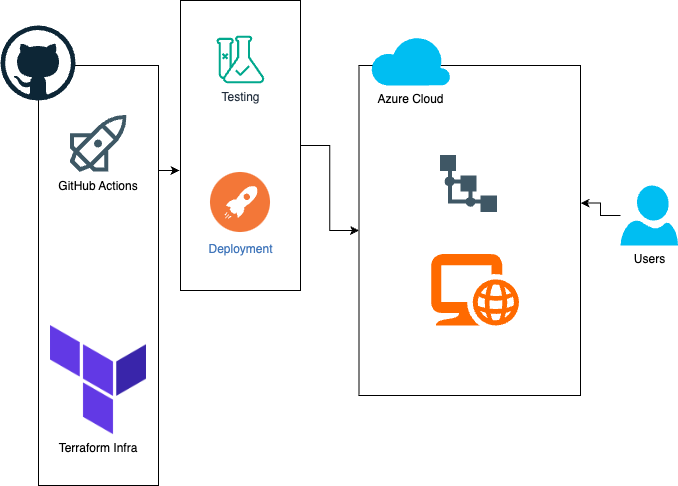
\includegraphics[width=0.5\textwidth]{../diagrams/AppStandard.drawio.png}
        \vspace{0.01\textwidth}
        \caption{Standard Configuration To Deploy An Application}
        \label{CloudStandard} % A unique label.
    \end{center}
\end{figure}


\subsection{Objectives of the Cloud Implementation of Webshop}

The Webshop is a critical component for LowTech GmbH, serving as the company’s primary sales platform. The goal of its cloud implementation is to enhance performance, scalability, and security, ensuring a seamless user experience.

Key objectives for the Webshop's cloud-based deployment include:

\begin{itemize}
    \item \textbf{Scalability and Performance Optimization:}
          The Webshop is deployed on Azure App Service with auto-scaling capabilities, enabling efficient traffic handling during peak periods. A load balancer ensures even traffic distribution across multiple instances.
          \bigskip % Adds space before the next section
    \item \textbf{High Availability and Reliability:}
          Azure Virtual Machine Scale Sets provide fault tolerance with automatic failover. Azure Blob Storage is used to securely store digital assets with high availability.
          \bigskip % Adds space before the next section
    \item \textbf{Security and Compliance:}
          The Webshop integrates with Microsoft Entra ID for user authentication and Azure Security Center for enhanced threat protection. Encryption and Role-Based Access Control (RBAC) are employed to safeguard sensitive customer data.
          \bigskip % Adds space before the next section
    \item \textbf{Continuous Deployment and DevOps Automation:}
          A CI/CD pipeline powered by GitHub Actions automates code deployments, improving deployment speed and reducing manual intervention.
          \bigskip % Adds space before the next section
    \item \textbf{Cost Efficiency and Resource Optimization:}
          The dynamic allocation of resources optimizes compute and storage usage, reducing operational expenses. Azure’s pay-as-you-go model aids in cost forecasting and budget management.
          \bigskip % Adds space before the next section
    \item \textbf{Future-Proofing and Cloud-Native Development:}
          The Webshop follows cloud-native best practicesn such as infrastructure as code, and continuous deployments.
\end{itemize}

\section{Application Design}
\subsection{Architectural Overview}
As requested by the project. This application wil have 3 tiers. The presentation or user interface, the backend or business logic, and the storage tier.
By our plan in milestone II we will deploy each tier in a different azure service tailored for its needs.
Each of the services provides autoscaling features, and load balancing. Ensuring that we are leveraging the elasticity charactersitics of the cloud.

\subsubsection{Presentation-Tier (Frontend) - User Interface (UI)}

It is important to note that the majority of the presentation was forked from https://github.com/DebasmitaMallick/React-e-Commerce-Website.
This allowed our team to focus on backend and cloud deployment tasks. The original project was modified to interact with our backend API,
integrate with payment providers and provide detailed information about products.

\paragraph{Technology Stack}
\begin{itemize}
    \item Frontend Framework: React.js (JavaScript)
    \item State Management: React Context API
    \item Hosting \& Deployment: Azure Static Web Apps
\end{itemize}

\paragraph{Functionality Overview}
\begin{enumerate}
    \item Navigation \& Routing
          Users can navigate between different sections of application, such as viewing product lists, accessing product details, and managing their shopping cart. React Router enables seamless client-side navigation.
          \begin{itemize}
              \item React Router Setup
                    \begin{itemize}
                        \item React Router (react-router-dom) to handle the routing of different components, allowing users to navigate through pages like the homepage (/), product detail pages (/product/:id), and potentially a shopping cart or checkout page.
                        \item For product detail pages, you're using dynamic routes with product/:id to fetch and display specific product data based on the product’s unique id. For instance:
                        \item When a user clicks on a product in the catalog, the URL changes to something like /product/123, and the ProductDetail component is rendered with data for product 123.
                        \item This is achieved using useNavigate and useParams hooks provided by React Router to capture the dynamic part of the URL.
                    \end{itemize}

              \item Navigation Links
                    \begin{itemize}
                        \item On the homepage (Home.js component), displaying a list of products. Each product has an image and name that users can click. When clicked, the app navigates to the product detail page using the navigate(/product/\${prod.id}) function
                    \end{itemize}
          \end{itemize}
    \item API Communication
          \begin{itemize}
              \item The product data, which includes the list of products with details such as images, names, prices, and categories, is fetched when the homepage or product catalog page loads.
                    This is done using useEffect to trigger an API call and update the state with the fetched data.
              \item API communication in app is responsible for sending and receiving data from the backend server. This includes fetching product data to populate catalog, and creating orders after checkout.
              \item For payment, we use PayPal and Stripe in a sandbox mode. As this is not the final product, we are just testing the actual integration with the providers.
          \end{itemize}

\end{enumerate}
\paragraph{Key Features of the UI}
\begin{enumerate}
    \item UI Components \& Design
          \begin{itemize}
              \item Key Features
                    \begin{itemize}
                        \item Reusable Components: Components like SingleProduct.js, ProductDetail.js, and Cart.js.
                        \item Bootstrap Integration: react-bootstrap is used to style UI components to enable responsive behavior.
                        \item Dark \& Light Theme Support: A theme context (ThemeContextProvider) dynamically adjusts UI styles based on user preference.
                    \end{itemize}
          \end{itemize}

    \item Product Display \& Interaction
          The UI displays products with details, allowing users to browse, select, and view product specifications before making a purchase.
          \begin{itemize}
              \item Key Features
                    \begin{itemize}
                        \item Product Catalog: Displays a grid of available products with images, names, and prices.
                        \item Product Cards (SingleProduct.js):
                              \begin{itemize}
                                  \item Clickable product images navigate to the product details page.
                                  \item Shows product information such as name, category, description, and price.
                                  \item ``Add to Cart'' and ''Remove from Cart'' buttons enable quick cart management.
                              \end{itemize}
                        \item Product Details Page (ProductDetail.js):
                              \begin{itemize}
                                  \item Displays full product details, including stock availability.
                                  \item Users can add/remove items from the cart.

                              \end{itemize}
                    \end{itemize}
          \end{itemize}

    \item Shopping Cart UI \& Checkout
          The cart and checkout sections provide a way for users to review their selected products and manage quantities.
          \begin{itemize}
              \item Key Features
                    \begin{itemize}
                        \item Cart UI (Cart.js)
                              \begin{itemize}
                                  \item Displays a list of selected products with prices and a ''Remove from Cart'' button.
                                  \item Updates total price dynamically based on the cart's contents.
                                  \item Navigates users to checkout when ready.
                              \end{itemize}
                        \item Checkout UI (CheckoutForm.js)
                              \begin{itemize}
                                  \item Collects user details (name, email, and shipping information).
                                  \item Integrates Stripe and PayPal for secure payment processing.
                                  \item Displays success messages with reference numbers for placed orders.
                              \end{itemize}
                    \end{itemize}
          \end{itemize}

    \item Notifications
          The app uses toast notifications and error messages to keep users informed.
          \begin{itemize}
              \item Key Features
                    \begin{itemize}
                        \item Toast Notifications (react-toastify)
                              \begin{itemize}
                                  \item Displays success messages when products are added/removed from the cart.
                                  \item Shows error messages if something goes wrong (e.g., out-of-stock products, payment failures).
                              \end{itemize}
                    \end{itemize}
          \end{itemize}
\end{enumerate}

\begin{figure}[H]
    \centering
    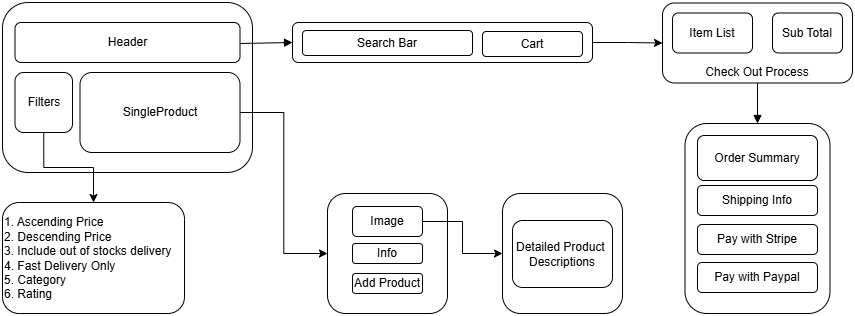
\includegraphics[width=0.6\textwidth]{../diagrams/componant diagram.drawio.png}
    \vspace{0.02\textwidth}
    \caption{Component Diagram}
    \label{fig:component_diagram}
\end{figure}

\subsubsection{Application-Tier (Backend) - Business Logic}
\paragraph{Technology Stack}
\begin{itemize}
    \item FastAPI
    \item SQLAlchemy
\end{itemize}

\paragraph{Product Management} \leavevmode

The Product Management module handles the lifecycle of products in the system. This includes operations for adding new products, updating product details, and retrieving product information. The core business logic ensures that products are categorized correctly, their stock levels are managed, and prices are updated as needed.
\begin{itemize}
    \item Key Operations:
          \begin{itemize}
              \item Add, update, and delete products.
              \item Manage product details such as descriptions, prices, and categories.
              \item Track stock availability and reorder levels.
          \end{itemize}
\end{itemize}

\paragraph{Order Management} \leavevmode

The Order Management module manages customer orders, from order creation, and status changes. It tracks the order status and ensures that orders are processed correctly.
\begin{itemize}
    \item Key Operations:
          \begin{itemize}
              \item Create and update orders with customer and product information.
              \item Monitor order statuses (e.g., processing, dispatched, delivered).
              \item Validate inventory and ensure product availability during order processing.
          \end{itemize}
\end{itemize}

\paragraph{Inventory Management} \leavevmode

The Inventory Management module tracks the stock levels of all products, ensuring that inventory can be updated.
\begin{itemize}
    \item Key Operations:
          \begin{itemize}
              \item Monitor and update product stock levels after each sale.
              \item Track the supplier’s stock.
          \end{itemize}
\end{itemize}

\paragraph{Email Notification} \leavevmode

The Email Notification module sends emails to customers and administrators for various events in the system, such as order confirmations, shipment tracking updates, and payment status notifications. It integrates with FastMail to send HTML-formatted emails with dynamic content.
\begin{itemize}
    \item Key Operations:
          \begin{itemize}
              \item Send order confirmation emails to customers.
              \item Notify customers of order status updates, such as dispatched or delivered.
              \item Alert suppliers of low stock levels and send reorder requests.
              \item Provide a user-friendly email template system for various types of notifications.
          \end{itemize}
\end{itemize}

\subsubsection{Data-Tier (Database) - Databases}
\paragraph{Technology Stack}
\begin{itemize}
    \item PostgreSQL
    \item Alembic
    \item Azure Database for PostgreSQL
\end{itemize}
\paragraph{Database}
\begin{enumerate}
    \item Product Data
          \begin{itemize}
              \item Product
                    \begin{itemize}
                        \item Stores the core product information and links to categories, suppliers, and inventory.
                        \item Key Attributes:
                              \begin{itemize}
                                  \item id: Unique product identifier (Primary Key).
                                  \item name: Product name.
                                  \item description: Product description.
                                  \item category\_id: Foreign Key linking to the Categories table.
                                  \item supplier\_id: Foreign Key linking to the Suppliers table.
                                  \item stock\_id: Links to the Stock table for inventory tracking.
                                  \item public\_unit\_price: Price displayed to customers.
                                  \item supplier\_unit\_price: Price from the supplier (for internal calculations).
                                  \item ean\_code: Unique product code for identification.
                                  \item reorder\_level: Threshold for restocking.
                                  \item img\_link: URL to the product image.
                                  \item extra\_info: JSON field to store additional product attributes. Like the ratings, or if the product has fast delivery.
                              \end{itemize}
                    \end{itemize}
              \item Catagories
                    \begin{itemize}
                        \item This table categorizes products for better organization and searchability.
                        \item Key Attributes:
                              \begin{itemize}
                                  \item id: Unique category identifier (Primary Key).
                                  \item name: Product name.
                                  \item description: Category description.
                                  \item extra\_info: JSON field for additional metadata.
                              \end{itemize}
                    \end{itemize}
          \end{itemize}

    \item Order Data
          \begin{itemize}
              \item Order
                    \begin{itemize}
                        \item This table records general order details and customer information.
                        \item Key Attributes:
                              \begin{itemize}
                                  \item id: Unique order identifier (Primary Key).
                                  \item customer\_name: Name of the customer.
                                  \item customer\_email: Customer's email address for notifications.
                                  \item customer\_phone: Contact number.
                                  \item order\_total: Total value of the order.
                                  \item status: Enum representing the order state (e.g., ''active'', ''cancelled'').
                                  \item tracking\_status: Enum tracking delivery progress (e.g., ''dispatched'', ''delivered'').
                                  \item payment\_method: JSON field storing payment details (e.g., card type).
                                  \item customer\_shipping\_info: JSON field for customer delivery address.
                                  \item created\_at: Timestamp when the order was created.
                                  \item updated\_at: Timestamp when the order was last updated.
                              \end{itemize}
                    \end{itemize}
              \item Order Details
                    \begin{itemize}
                        \item This table provides itemized details of each product within an order.
                        \item Key Attributes:
                              \begin{itemize}
                                  \item id: Unique identifier for each order detail record (Primary Key).
                                  \item order\_id: Foreign Key linking to the Orders table.
                                  \item product\_id: Foreign Key linking to the Products table.
                                  \item quantity: Number of units of the product ordered.
                                  \item product\_price: Unit price at the time of the order.
                                  \item subtotal: Calculated subtotal for the item.

                              \end{itemize}
                    \end{itemize}
          \end{itemize}

    \item Inventory Data
          \begin{itemize}
              \item Stocks
                    \begin{itemize}
                        \item Monitors the available quantity of each product and manages restocking.
                        \item Key Attributes:
                              \begin{itemize}
                                  \item id: Unique stock identifier (Primary Key).
                                  \item quantity: Number of available units for a product.
                                  \item updated\_at: Timestamp of the last stock update.
                                  \item created\_at: Timestamp when the stock record was created.

                              \end{itemize}
                    \end{itemize}
              \item Suppliers
                    \begin{itemize}
                        \item Manages supplier-related information and links to products for procurement.
                        \item Key Attributes:
                              \begin{itemize}
                                  \item id: Unique supplier identifier (Primary Key).
                                  \item name: Supplier name.
                                  \item address: Supplier’s physical address.
                                  \item phone: Contact number.
                                  \item email: Contact email address.

                              \end{itemize}
                    \end{itemize}
          \end{itemize}
    \item  Database Migrations with Alembic
          \begin{itemize}
              \item It allows us to track database changes, apply updates to production, and roll back changes when needed.
              \item Key Operations with Alembic:
                    \begin{itemize}
                        \item \textit{Schema Migration:} Automatically generates migration scripts to apply changes to the database (e.g., adding new fields to a table).
                        \item \textit{Version Control:} Each migration is versioned, allowing us to track and audit changes.
                        \item \textit{Rollback Support:} Provides the ability to downgrade to previous schema versions if issues arise.
                    \end{itemize}
          \end{itemize}
\end{enumerate}

\begin{figure}[H]
    \centering
    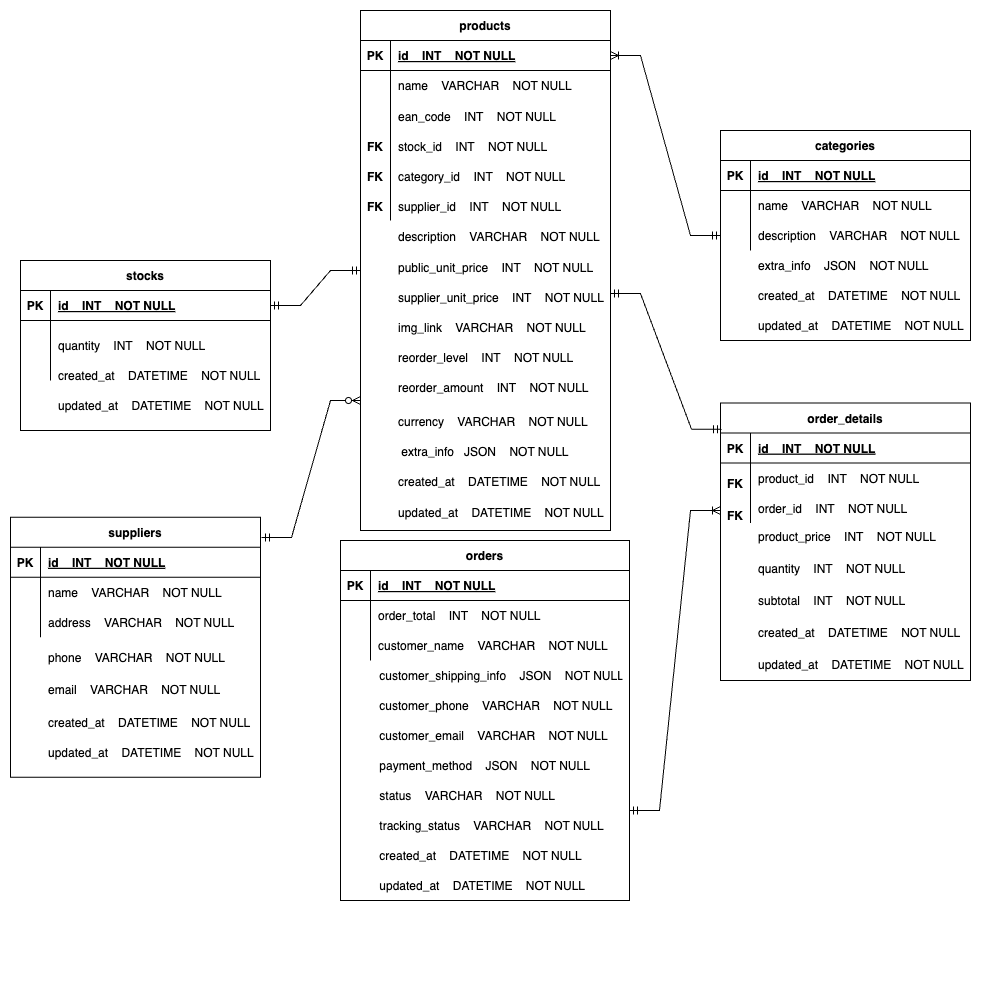
\includegraphics[width=0.6\textwidth]{../diagrams/webshop_erd.drawio.png}
    \caption{ERD Diagram of the Webshop Database}
    \label{fig:erd_webshop}
\end{figure}

\subsection{Development Process}

For the development of the application, the team created a Trello board. Using a kamban-like approach, we scoped,
divided, and prioritized all the necesary development and documentation tasks. Internally two teams were formed, frontend and backend.
Each working in a different layer of the webshop. The backend team was also in charge of the data layer just for convenience.
The most important tasks were to upgrade the existing UI code to fit the new requirements and integrate with the backend, and to actually develop the backend.
Frameworks like FastAPI were chosen due to the flexibility benefits, rapid development, and automatic documentation generation. Which allowed our team members to quickly review the spec and make the integration.
During the development timeline, we scheduled weekly meetings to report progress and address concearns with the development environment.

For example, we encountered issues while running the new `psycopg` libary in asynchronous mode in windows. Which caused some issues while configuring the development environment.
This could have been an oportunity to build a docker image to standardize our development environments, but given the timeline, we decided against it and changed to `asyncpg` in windows \\

\begin{figure}[H]
    \begin{center}
        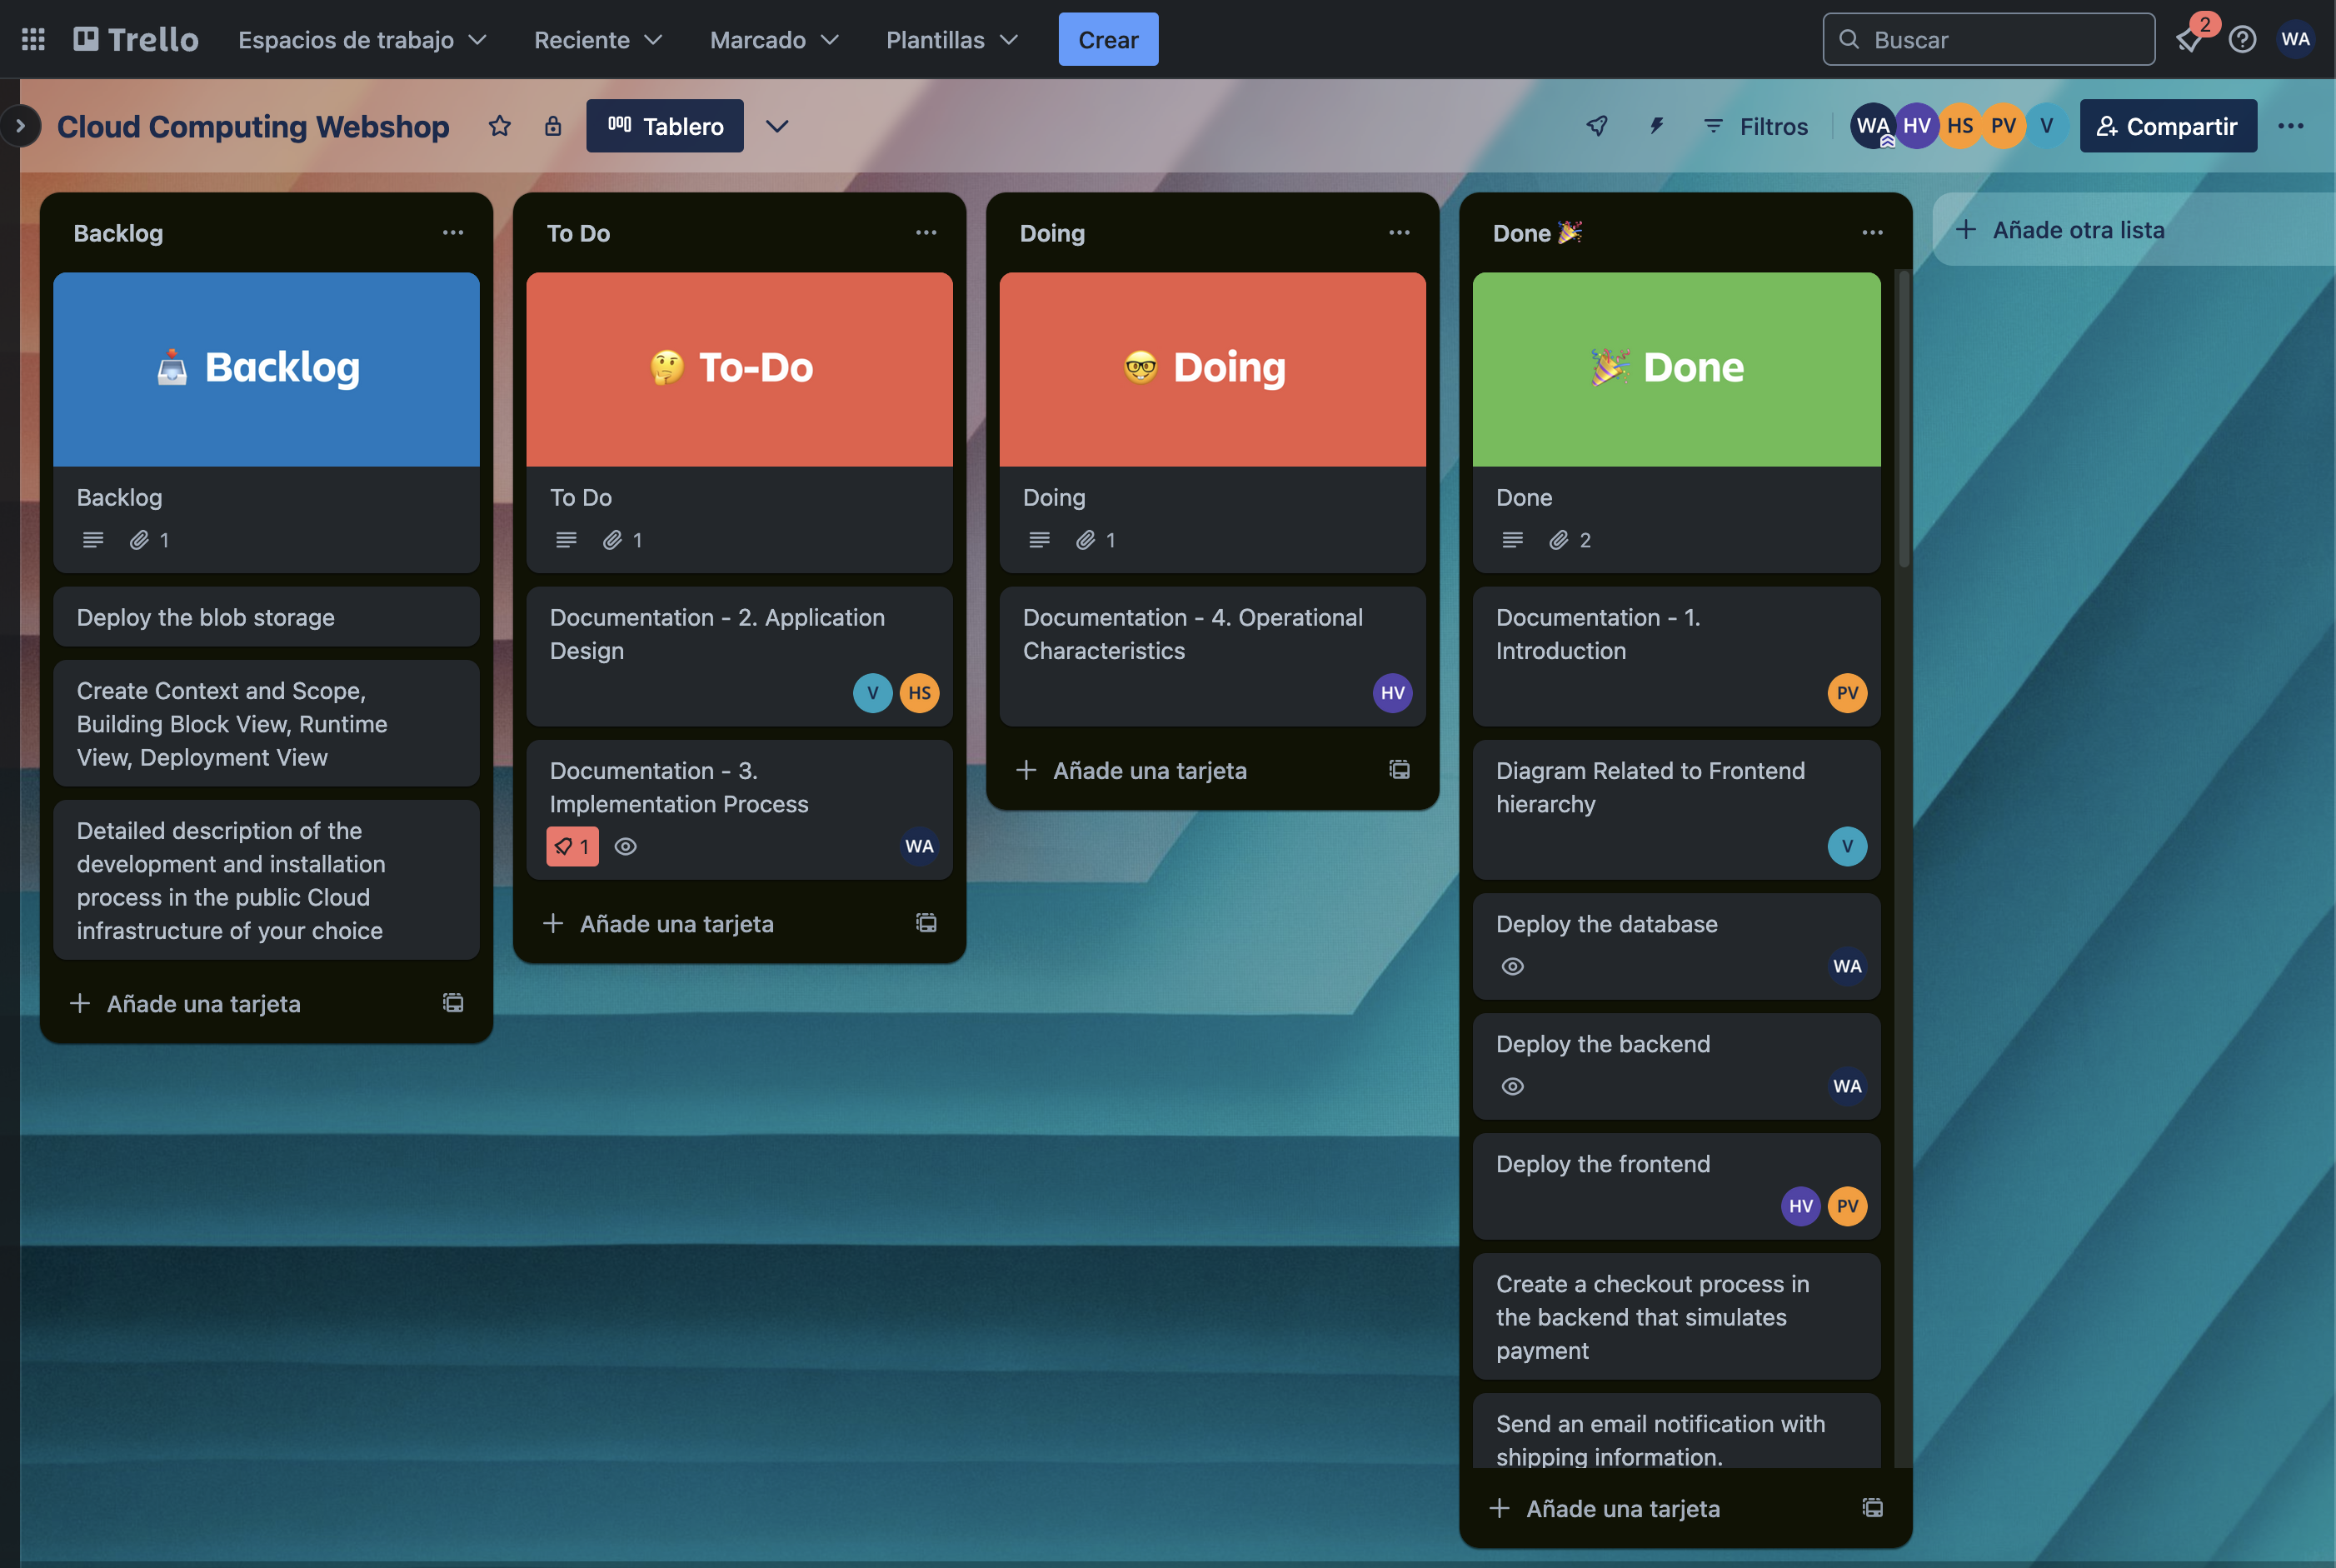
\includegraphics[width=0.7\textwidth]{../diagrams/trello_board.png}
        \vspace{0.01\textwidth}
        \caption{Trello Board}
        \label{TrelloBoard} % A unique label.
    \end{center}
\end{figure}
\section{System Diagrams}

\subsection{Context and Scope}
\begin{figure}[H]
    \begin{center}
        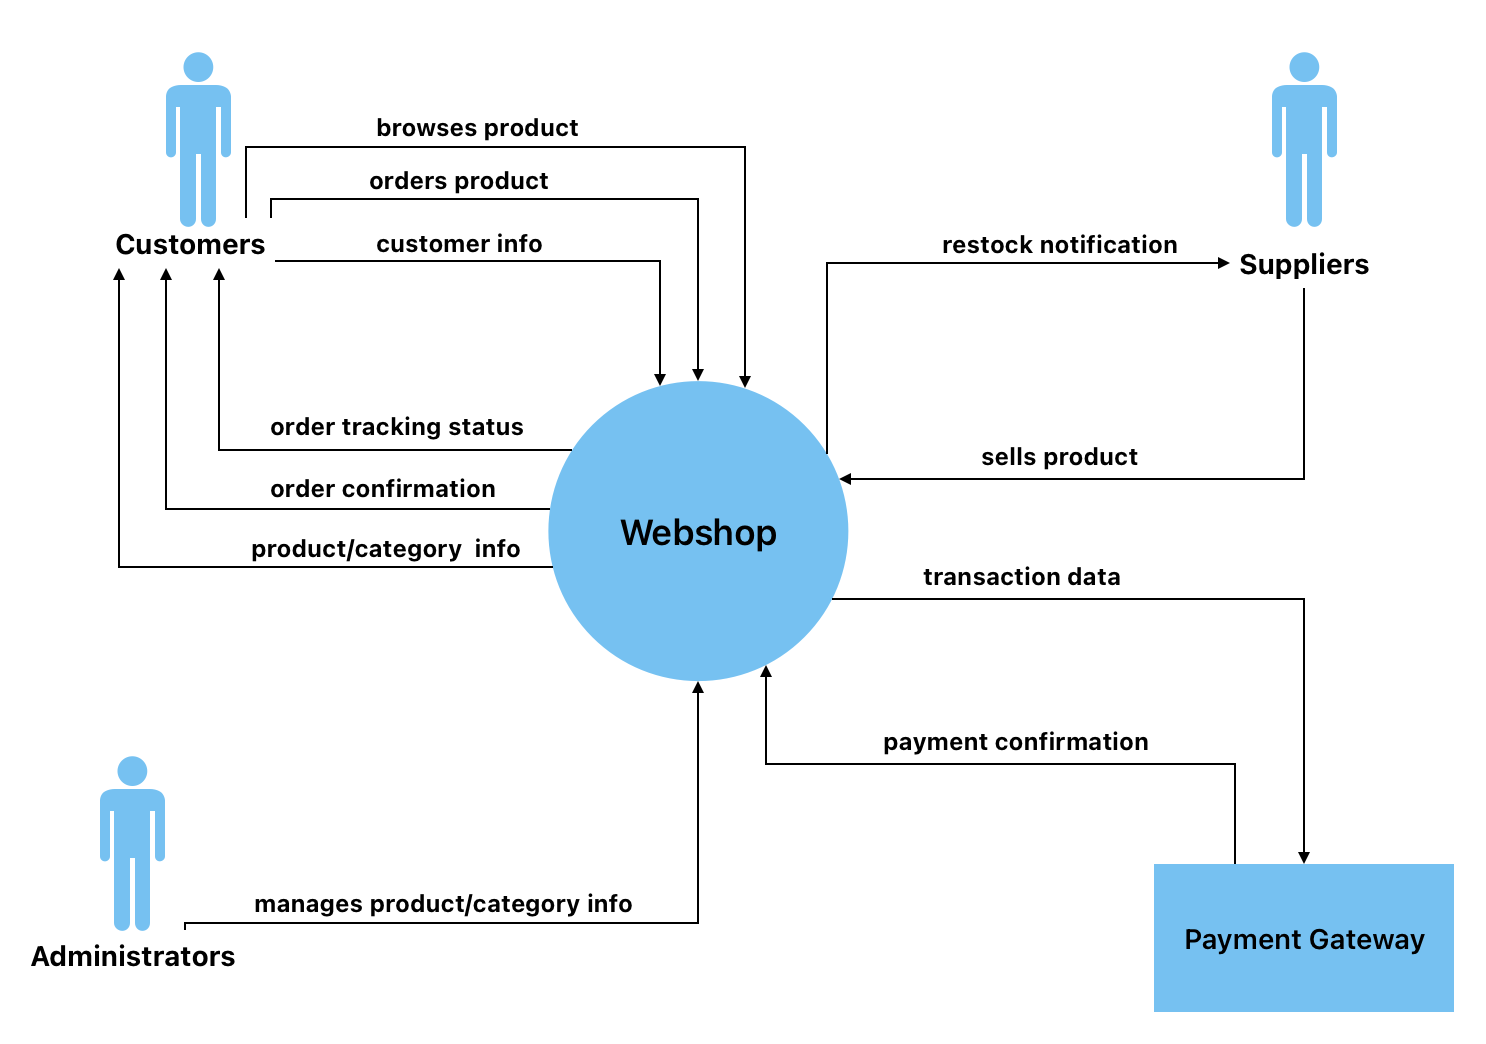
\includegraphics[width=0.8\textwidth]{../diagrams/contextview.png}
        \vspace{0.01\textwidth}
        \caption{Context and Scope Diagram}
        \label{ContextandScope} % A unique label.
    \end{center}
\end{figure}

\subsection{Building Block View}

\begin{figure}[H]
    \begin{center}
        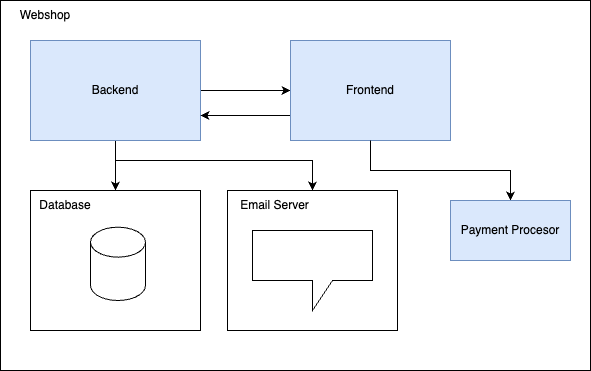
\includegraphics[width=0.9\textwidth]{../diagrams/block_diagram-Level1.drawio.png}
        \vspace{0.01\textwidth}
        \caption{Building Block View Level 1}
        \label{BuildingBlockView1}
    \end{center}
\end{figure}

The building block view makes emphasis on the backend, since we have provided a component diagram for the frontend.\\


\begin{figure}[H]
    \begin{center}
        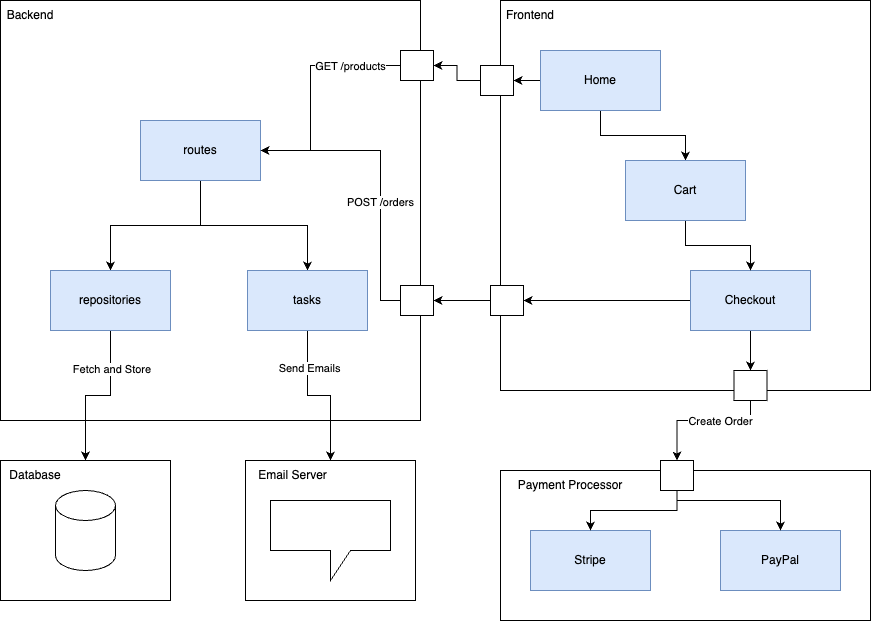
\includegraphics[width=0.9\textwidth]{../diagrams/block_diagram-Level2.drawio.png}
        \vspace{0.01\textwidth}
        \caption{Building Block View Level 2}
        \label{BuildingBlockView2}
    \end{center}
\end{figure}


\begin{figure}[H]
    \begin{center}
        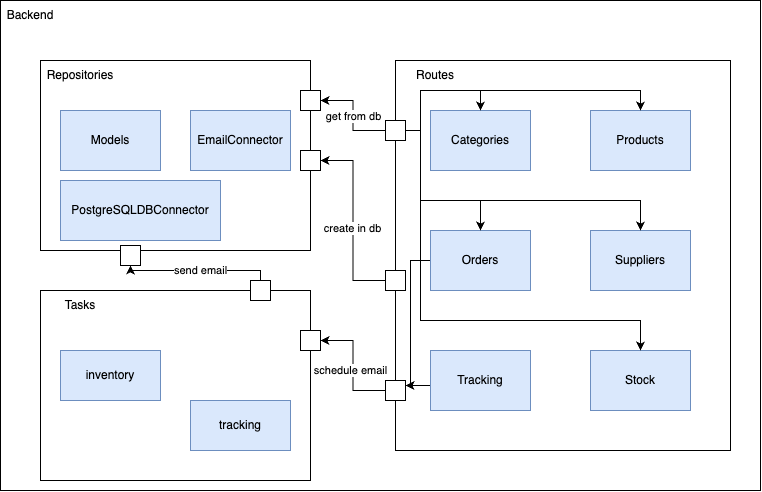
\includegraphics[width=0.9\textwidth]{../diagrams/block_diagram-Level3.drawio.png}
        \vspace{0.01\textwidth}
        \caption{Building Block View Level 3}
        \label{BuildingBlockView3}
    \end{center}
\end{figure}


\subsection{Runtime View}
\begin{figure}[H]
    \begin{center}
        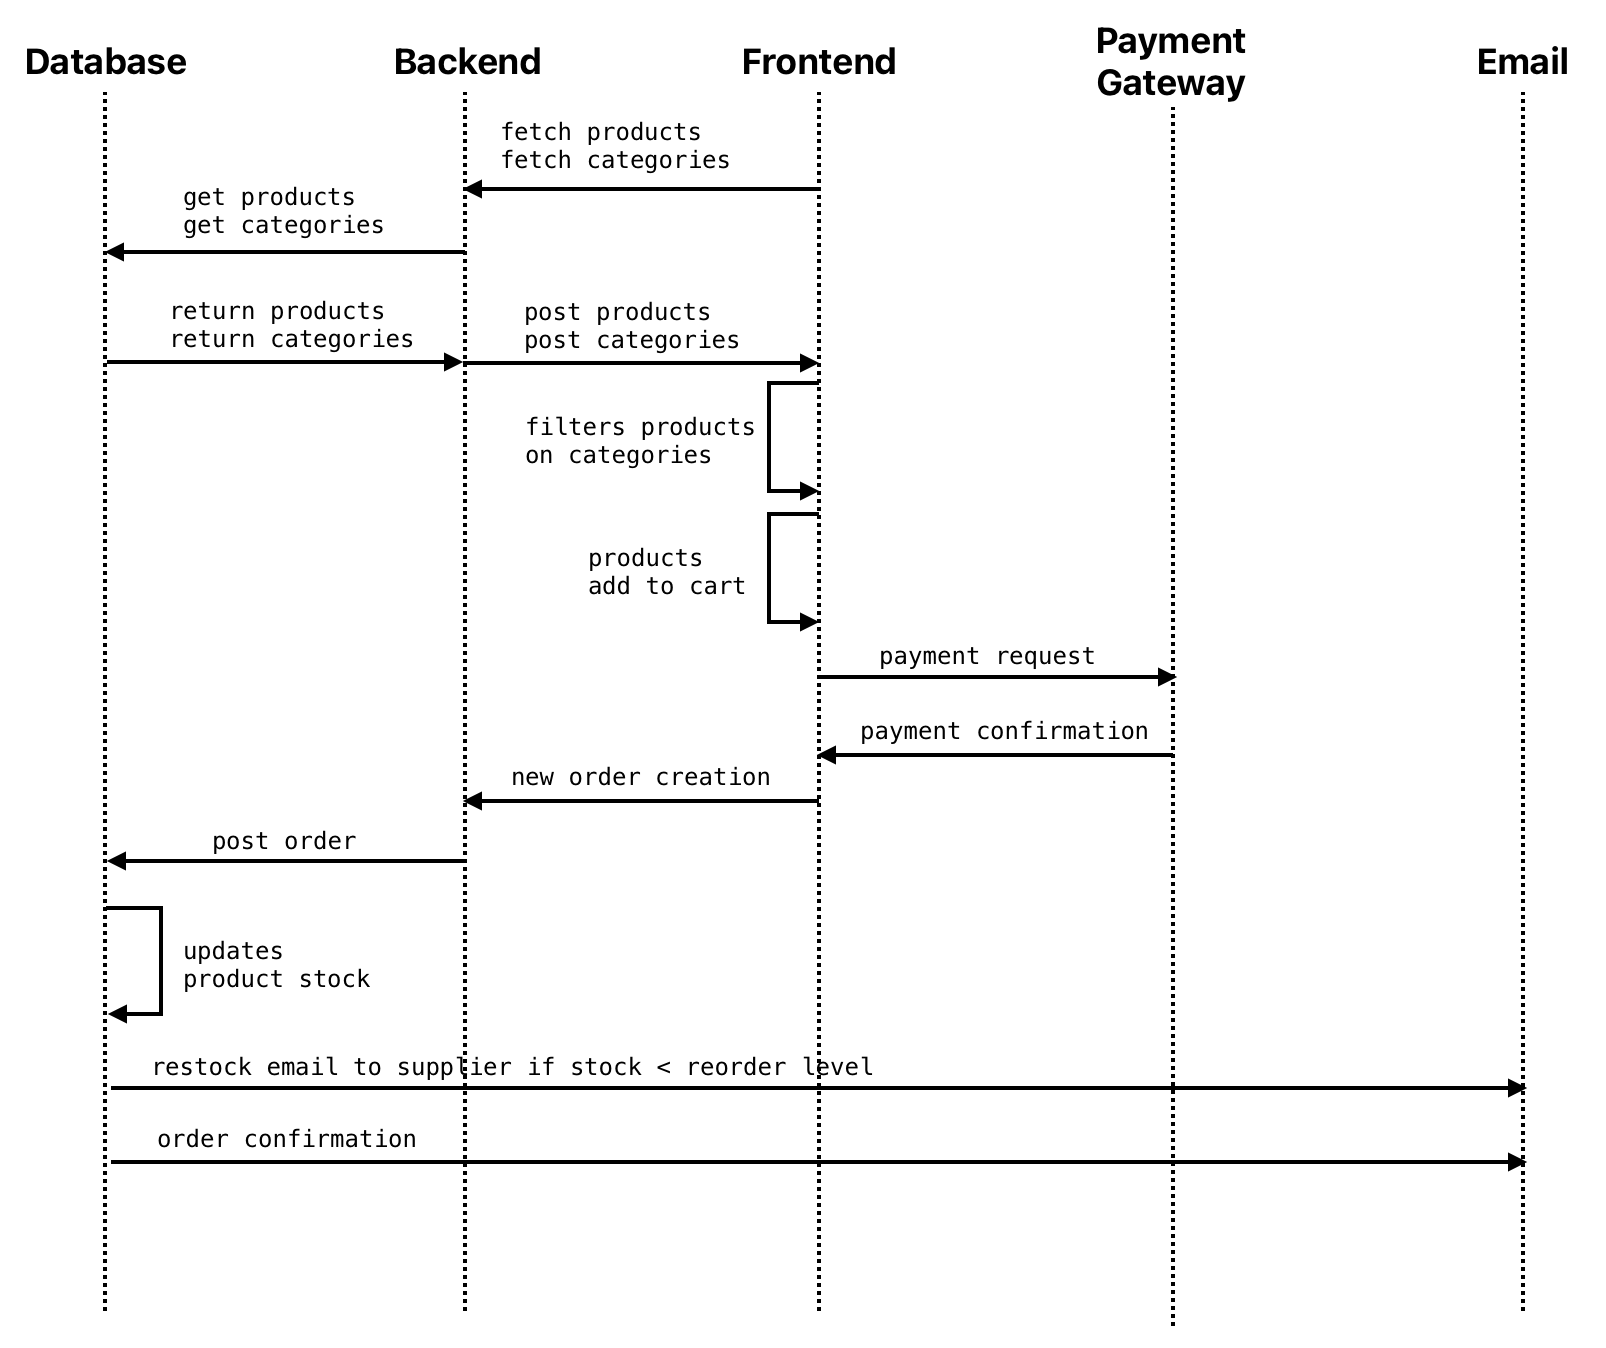
\includegraphics[width=0.9\textwidth]{../diagrams/runtimeview.png}
        \vspace{0.01\textwidth}
        \caption{Runtime View Diagram}
        \label{RuntimeView} % A unique label.
    \end{center}
\end{figure}


\subsection{Deployment View}

\begin{figure}[H]
    \begin{center}
        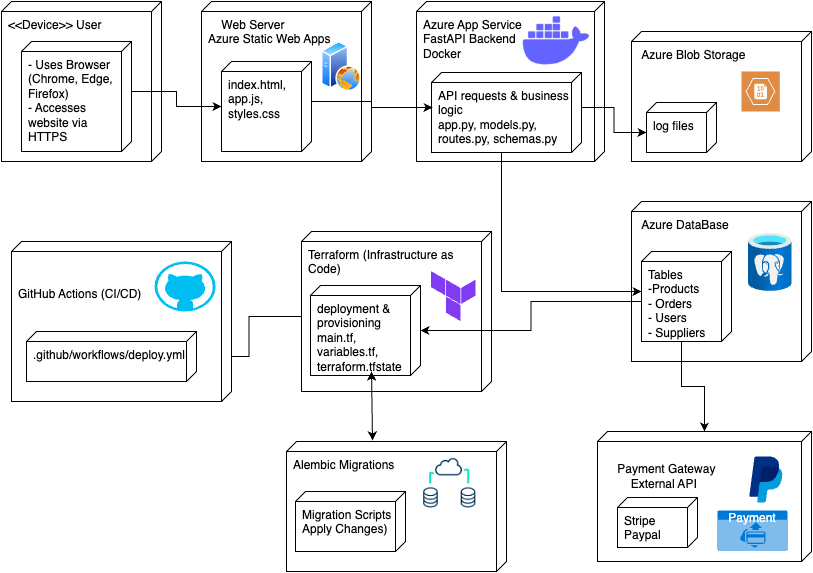
\includegraphics[width=0.7\textwidth]{../diagrams/deployment.png}
        \vspace{0.01\textwidth}
        \caption{Deployment View Diagram}
        \label{DeploymentView} % A unique label.
    \end{center}
\end{figure}


\section{Implementation Process}

To make the implementation easier and repeatable in the public cloud provider we used terraform.
Each of the different services was encapsulated in a module, allowing us to make the main template readable.
So far we did not setup any CI implementation for the infrastructure deploy, only for the code changes, since that the functionality was provided by Azure.

In the following code snippets we can see the specific infrastructure template we used for our deploy.

\begin{itemize}

    \item Configuration of the azure terraform provider:
          \lstinputlisting[lastline=19]{../../../infra/main.tf}
    \item Creation of a general resource group in Germany West Central (This zone is allowed by the student subscription)
          \lstinputlisting[firstline=20, lastline=24]{../../../infra/main.tf}
    \item Creation of a virtual network to comunicate the database and backend. This is required by the postgresql flexible server
          \lstinputlisting[firstline=25, lastline=68]{../../../infra/main.tf}
    \item Creation of a private DNS zone for the database. This is required to get an internal DNS name avoiding the use of a single public IP.
          \lstinputlisting[firstline=70, lastline=84]{../../../infra/main.tf}
    \item Creation of the DB, frontend and backend modules. All necesary code is included in the /infra folder of the repository.
          \lstinputlisting[firstline=84]{../../../infra/main.tf}
\end{itemize}

To get the appropriate credentials, we created a student account with 100USD in credits, after running the
$\verb|az ad sp create-for-rbac --role="Contributor" --scopes="/subscriptions/<SUBSCRIPTION_ID>"|$ command
the team was able to populate the respective variables file. Finally we executed the terraform plan to create the infrastructure.\\

\begin{lstlisting}[language=Python,caption={Azure Credentials Example}]
    {
        "appId": "XXXXX-XXXX-XXX-XXX-XXXXXXX",
        "displayName": "azure-cli-2025-02-09-15-07-35",
        "password": "SECRET_PASSWORD",
        "tenant": "TENANT_UUID"
    }
\end{lstlisting}

\begin{figure}[H]
    \begin{center}
        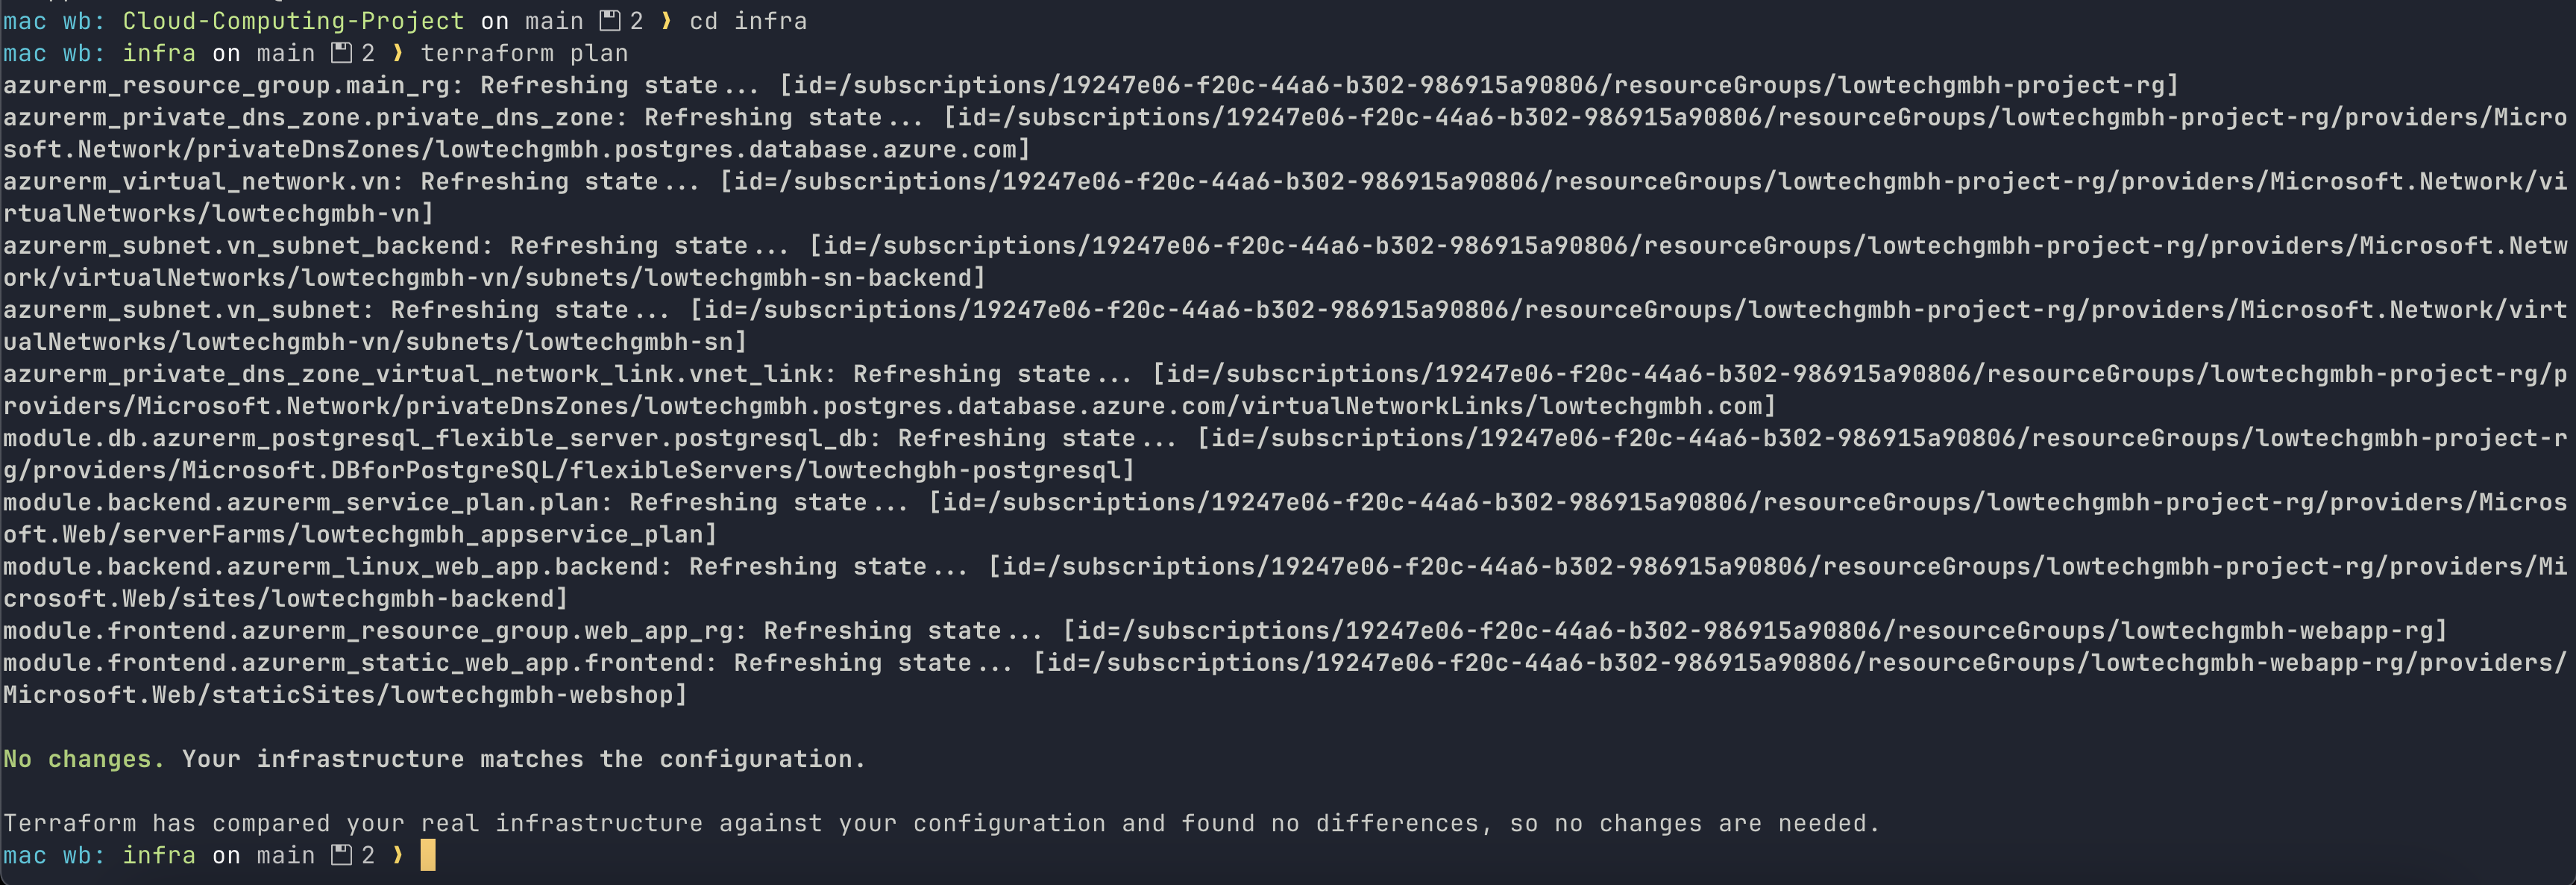
\includegraphics[width=0.7\textwidth]{../images/terraform_plan.png}
        \vspace{0.01\textwidth}
        \caption{Terraform Plan Results}
        \label{TerraformPlan} % A unique label.
    \end{center}
\end{figure}

\subsection{Cloud Environment Setup}


Once we had all resources created in Azure, the team had to perform further manual configurations to enable the CI pipelines in azure webapps and static websites.
\begin{itemize}
    \item To enable CI for the backend we used the provided azure functionality which created a GitHub actions file wich packages and uploads all changes once they are merged into main
    \item To enable CI for the frontend we used the provided azure functionality, which esentially provides the same features as in the backend.
    \item We also created an standalone virtual machine with access to the database, in this virtual machine we ran all migrations and seeded the database si all data was available for testing.\\
\end{itemize}

\begin{figure}[H]
    \begin{center}
        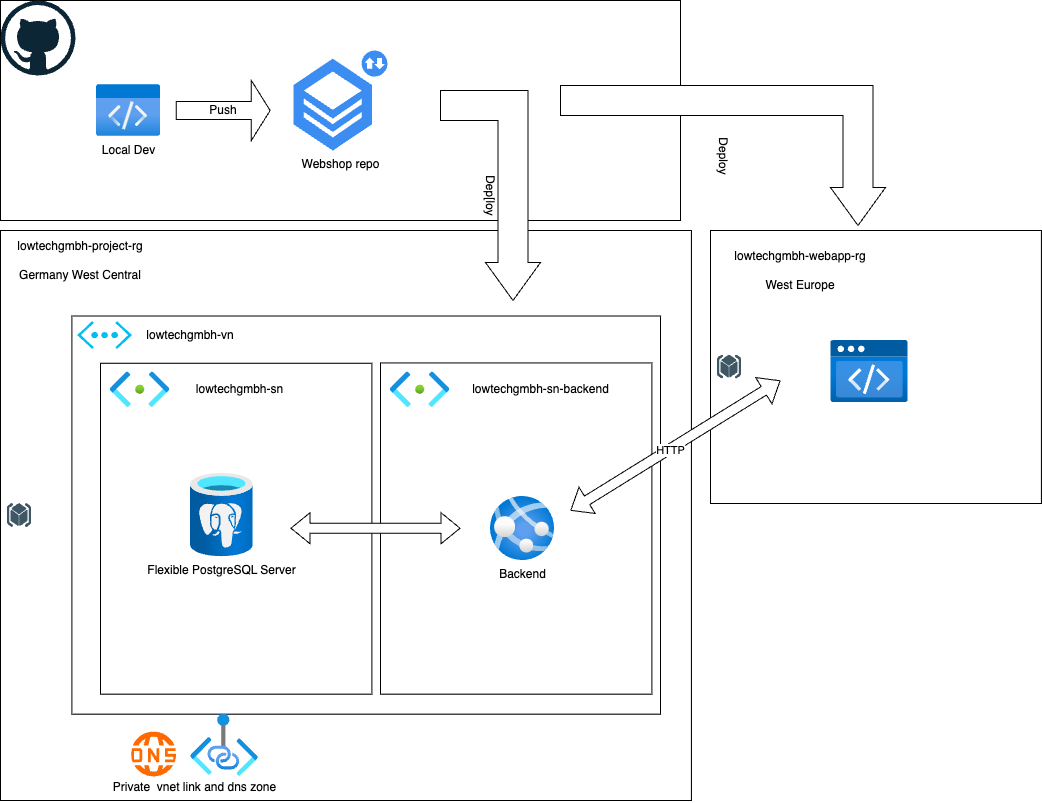
\includegraphics[width=0.7\textwidth]{../diagrams/webapp_tf_azure.drawio.png}
        \vspace{0.01\textwidth}
        \caption{Cloud Environment Setup Diagram}
        \label{CloudSetup} % A unique label.
    \end{center}
\end{figure}



\subsection{Development Challenges}
\begin{itemize}
    \item Sometimes the azure terraform provider encountered race conditions and produced errors while creating or destroying the infrastructure.
    \item Some functionalities are not available for the student subscription, so we had to change availavility zones until we got one that was allowed
    \item By default our applications don't have any autoscaling configured, given the choico of SKUs and to save costs.
          Nevertheless the functionallity can be enabled by changing one configuration in the dashboard
\end{itemize}

\section{Application Functionality and Characteristics}

\subsubsection{Functional Test Cases}

\renewcommand{\arraystretch}{1.3}
\begin{longtable}{|c|>{\raggedright}p{4.8cm}|p{6cm}|>{\centering\arraybackslash}p{2cm}|}
    \hline
    \textbf{Test Case ID} & \textbf{Test Scenario}                     & \textbf{Expected Outcome}                                 & \textbf{Status (Pass/Fail)}                   \\ \hline
    \endfirsthead
    \hline
    \textbf{Test Case ID} & \textbf{Test Scenario}                     & \textbf{Expected Outcome}                                 & \textbf{Status (Pass/Fail)}                   \\ \hline
    \endhead
    TC-001                & Load Homepage and verify product listing   & Homepage loads with products displayed correctly.         & Pass, see Figure \ref{fig:homepage_filters}   \\ \hline
    TC-002                & Apply Price filter (Ascending/Descending)  & Products reorder correctly based on selected price.       & Pass, see Figure \ref{fig:homepage_filters}   \\ \hline
    TC-003                & Apply Out of Stock filter                  & Only out-of-stock items are displayed.                    & Pass, see Figure \ref{fig:homepage_filters_2} \\ \hline
    TC-004                & Apply Fast Delivery filter                 & Only products eligible for fast delivery show up.         & Pass, see demo video        \\ \hline
    TC-005                & Filter by Category                         & Products are filtered correctly by selected category.     & Pass, see demo video       \\ \hline
    TC-006                & Search Product by Name or Category         & Products matching search are shown correctly.             & Pass, see demo video        \\ \hline
    TC-007                & Clear Filter functionality                 & All filters are removed, showing the full product list.   & Pass, see demo video        \\ \hline
    TC-008                & Product Detail Page - Click Product        & Clicking a product opens its detailed page.               & Pass, see demo video        \\ \hline
    TC-009                & Product Detail Page - Load Product Details & Product details (name, description, price) are displayed. & Pass, see demo video         \\ \hline
    TC-010                & Add a Product to Cart                      & Product appears in cart with correct details.             & Pass, see Figure \ref{fig:Webshop_3}         \\ \hline
    TC-011                & Increase product quantity in cart          & Quantity updates and is reflected in the cart.            & Pass, see Figure \ref{fig:Webshop_4}           \\ \hline
    TC-012                & Remove product from cart                   & Product is removed from the cart immediately.             & Pass, see Figure \ref{fig:Webshop_5}           \\ \hline
    TC-013                & Proceed to checkout                        & Checkout page loads with the correct order summary.       & Pass, see demo video         \\ \hline
    TC-014                & Select payment method - Stripe             & Stripe payment option is selected and processed.          & Pass, see Figure \ref{fig:Webshop_9}           \\ \hline
    TC-015                & Select payment method - PayPal             & PayPal payment option is selected and processed.          & Pass, see Figure \ref{fig:Webshop_6}           \\ \hline
    TC-016                & Complete order processing                  & Order confirmation message is displayed.                  & Pass, see demo video         \\ \hline
    TC-017                & Order confirmation email is received       & Email is sent after order is placed.                      & Pass, see Figure \ref{fig:Webshop_9}           \\ \hline
    TC-018                & Shipment notification email is received    & Email is sent when the order is shipped.                  & Pass, see Figure \ref{fig:Webshop_7}           \\ \hline
    TC-019                & Product Dispatched email is received       & Email is sent when the order is dispatched.               & Pass, see Figure \ref{fig:Webshop_8}           \\ \hline
    \caption{Functional Test Cases for Webshop} \label{tab:functional-test-cases}
    % \vspace{-10mm}
\end{longtable}



\textbf{Screenshots of the webshop}\\
\begin{figure}[H]
    \centering
    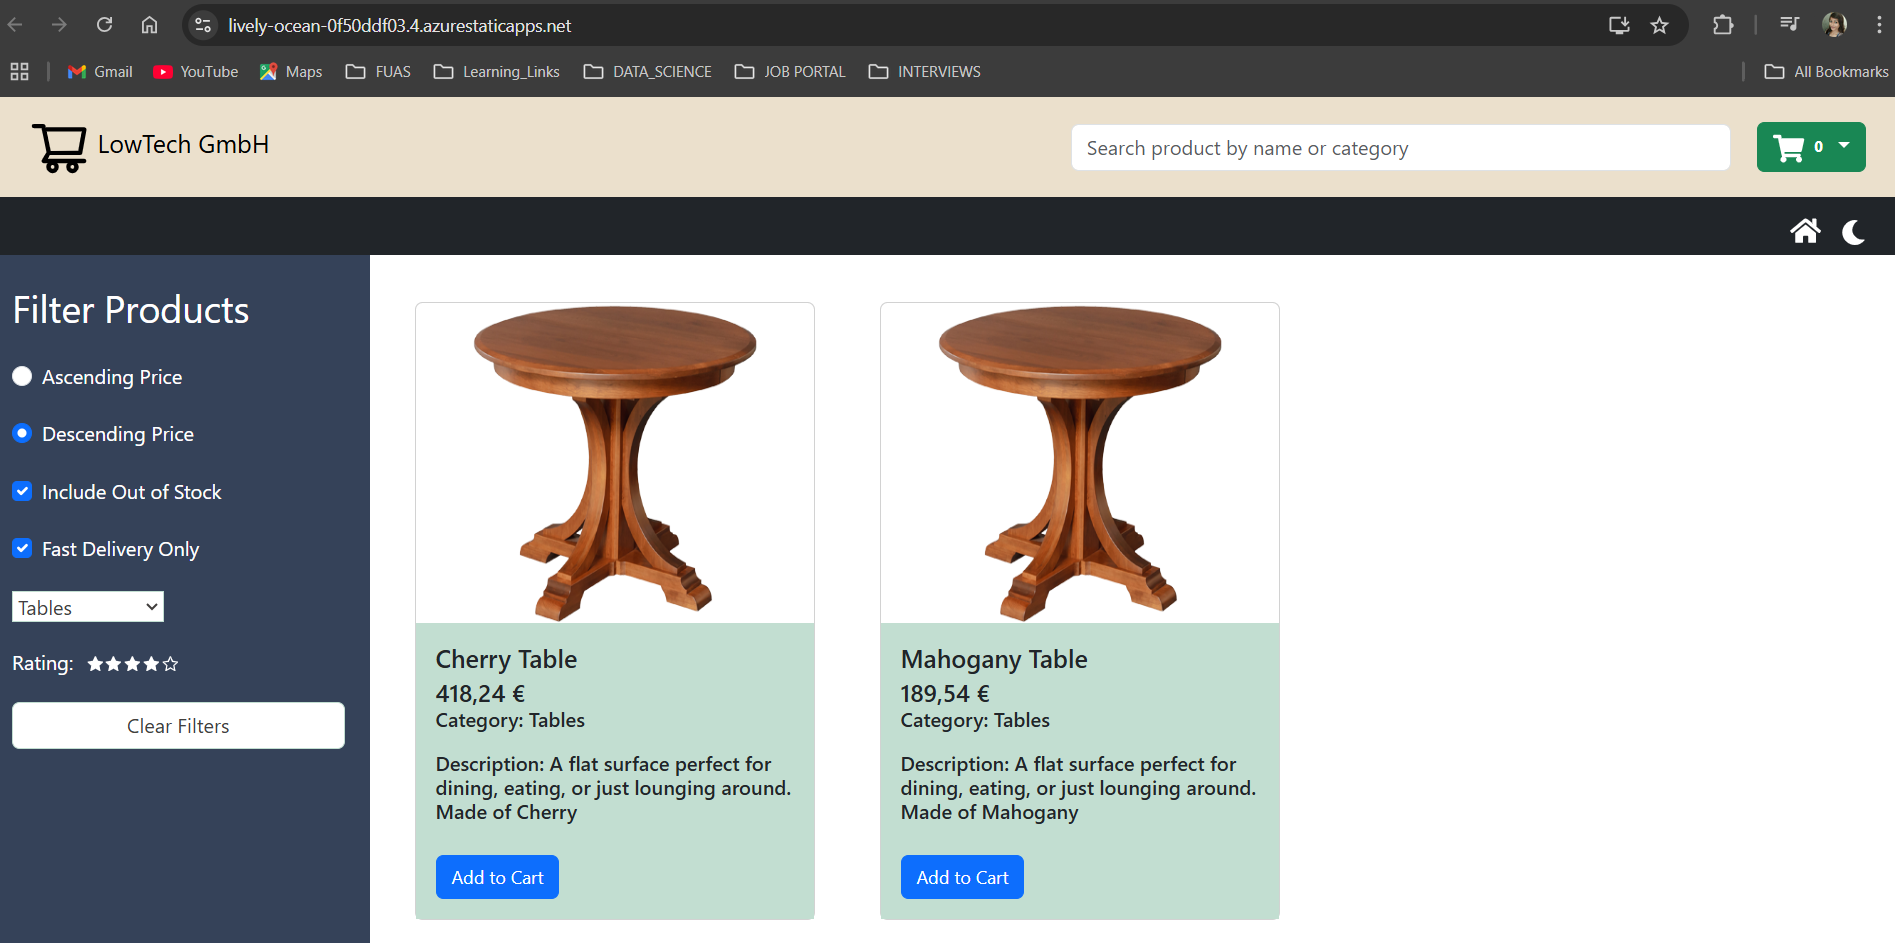
\includegraphics[width=0.8\textwidth]{../images/HomePage_AppliedFilters.png}
    \vspace{0.01\textwidth}
    \caption{Homepage with All Filters Applied to Products}
    \label{fig:homepage_filters}
\end{figure}

\vphantom{ }\\

\begin{figure}[H]
    \centering
    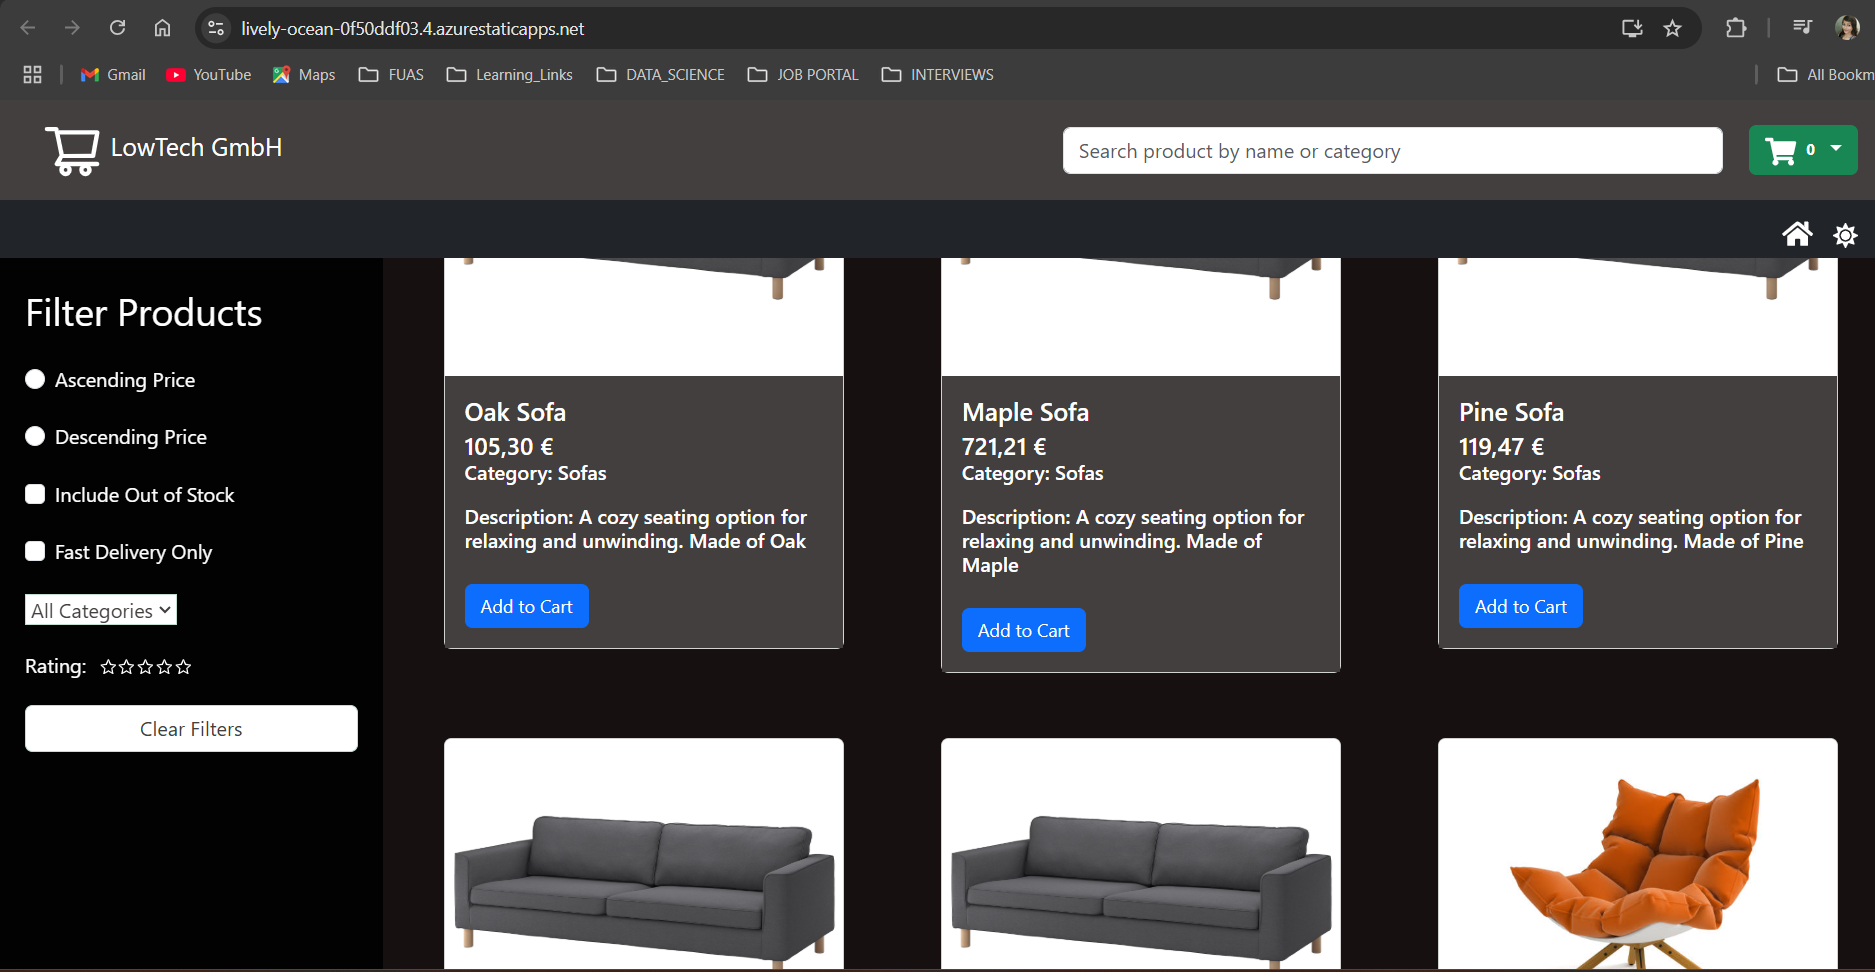
\includegraphics[width=0.8\textwidth]{../images/DarkTheme_Load.png}
    \vspace{0.01\textwidth}
    \caption{Homepage with All Products Listed, Dark Theme Enabled, and Clear Filter Applied}
    \label{fig:homepage_filters_2}
\end{figure}

\vphantom{ }\\

\begin{figure}[H]
    \centering
    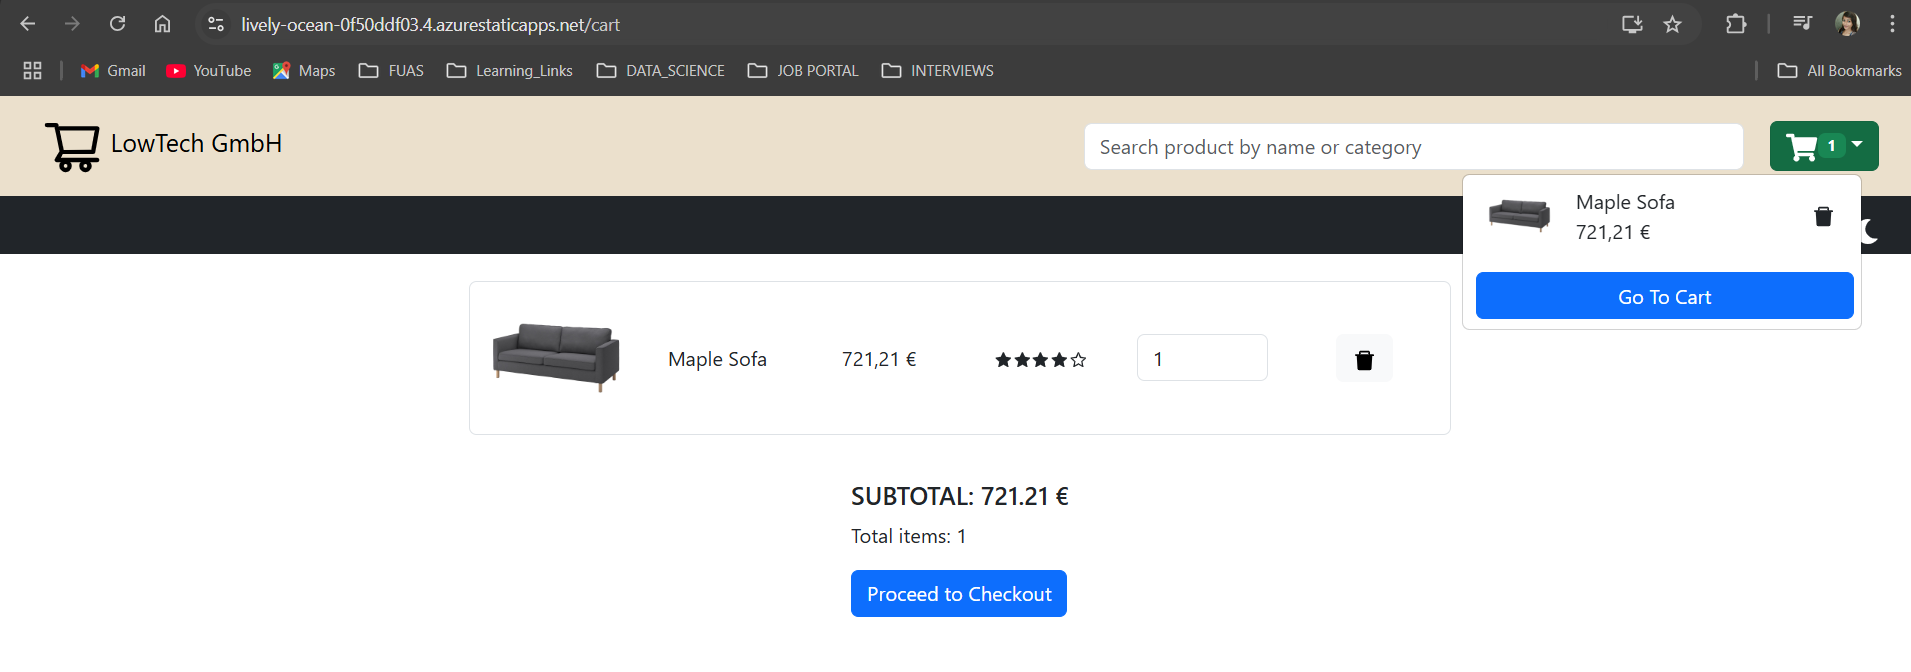
\includegraphics[width=0.8\textwidth]{../images/Item_Added_Cart.png}
    \vspace{0.01\textwidth}
    \caption{Product Added to Cart, Cart View Displayed with Selected Item}
    \label{fig:Webshop_3}
\end{figure}

\vphantom{ }\\
\begin{figure}[H]
    \centering
    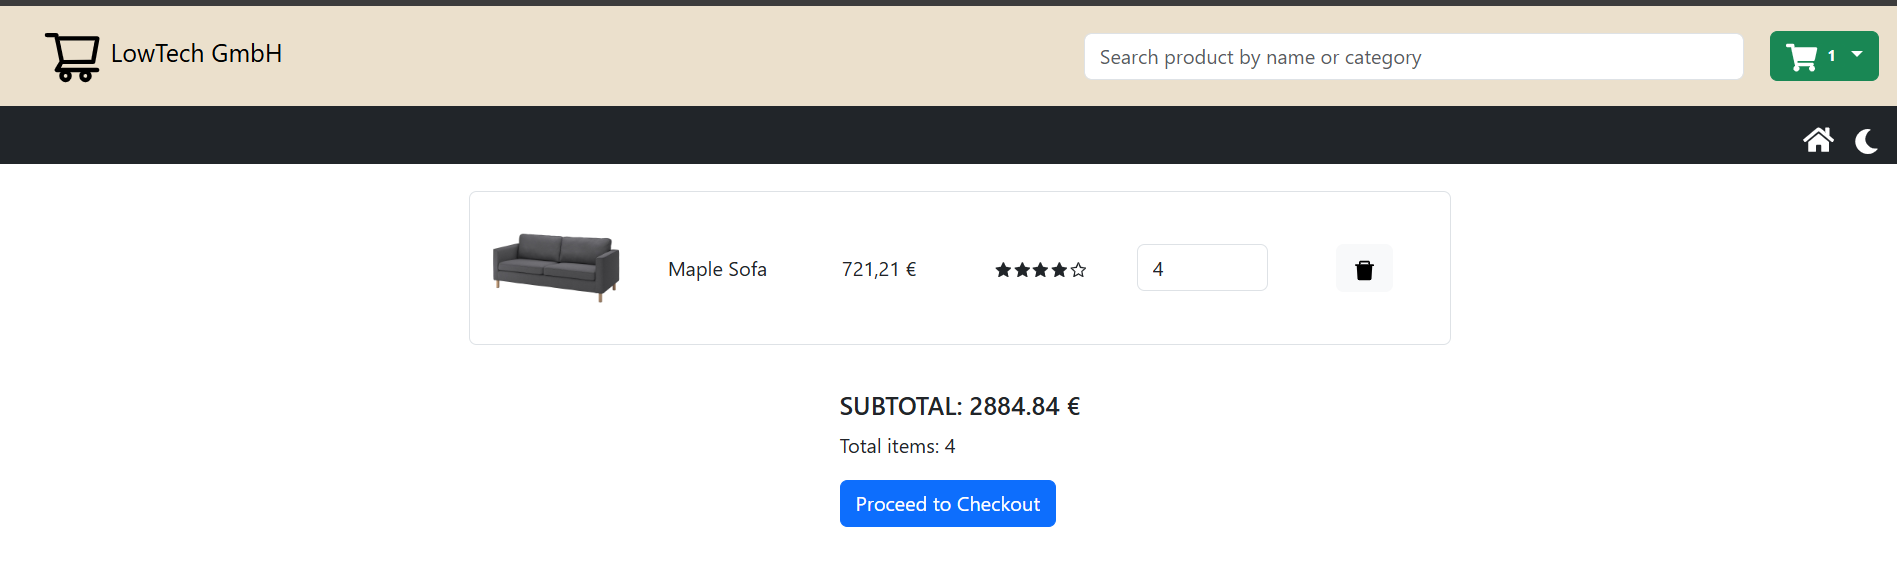
\includegraphics[width=0.8\textwidth]{../images/Cart_Item_Increase.png}
    \vspace{0.01\textwidth}
    \caption{Product Quantity Updated in Cart}
    \label{fig:Webshop_4}
\end{figure}
\vphantom{ }\\
\begin{figure}[H]
    \centering
    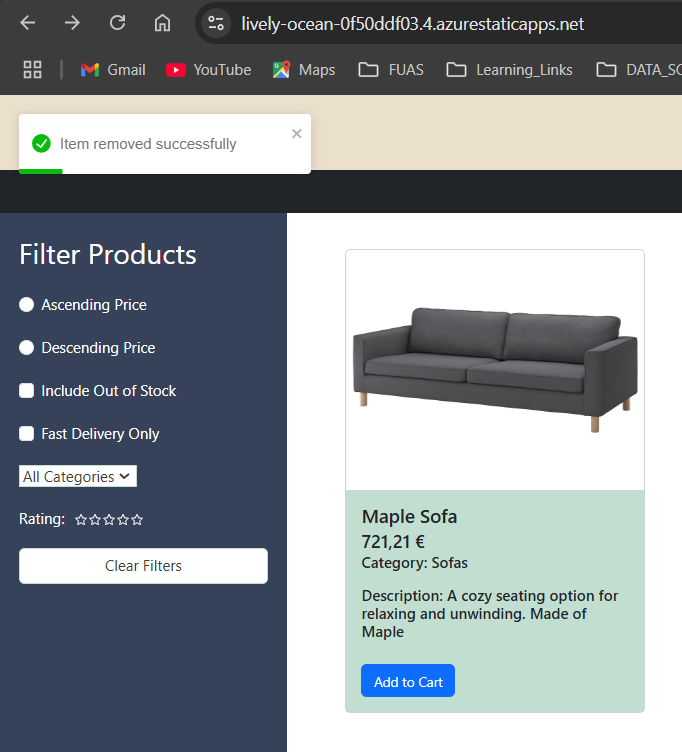
\includegraphics[width=0.4\textwidth]{../images/Item_remove_from_cart.png}
    \vspace{0.01\textwidth}
    \caption{Product Removed from Cart Successfully}
    \label{fig:Webshop_5}
\end{figure}

\vphantom{ }\\

\begin{figure}[H]
    \centering
    \subfloat[\centering Page Load]{{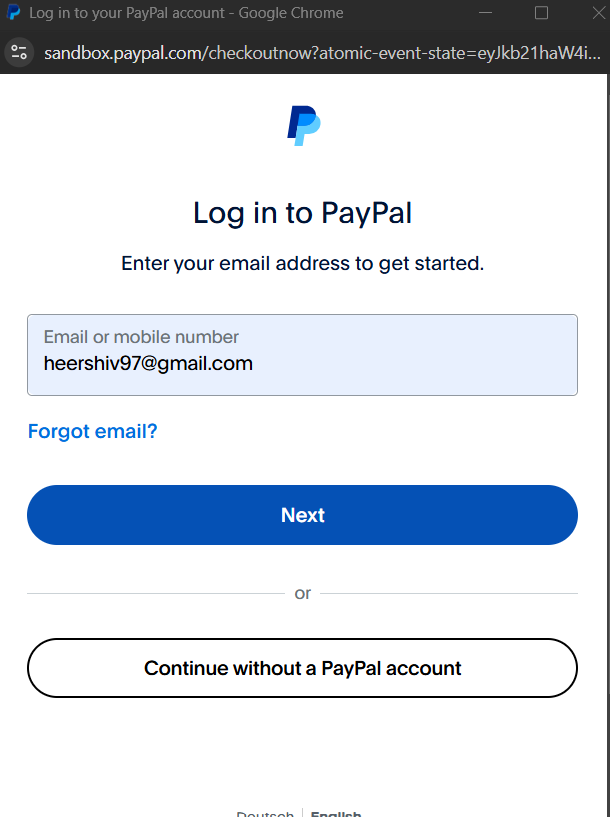
\includegraphics[width=0.4\textwidth]{../images/Paypal_Login.png} }}
    \qquad
    \subfloat[\centering Credit Card Input]{{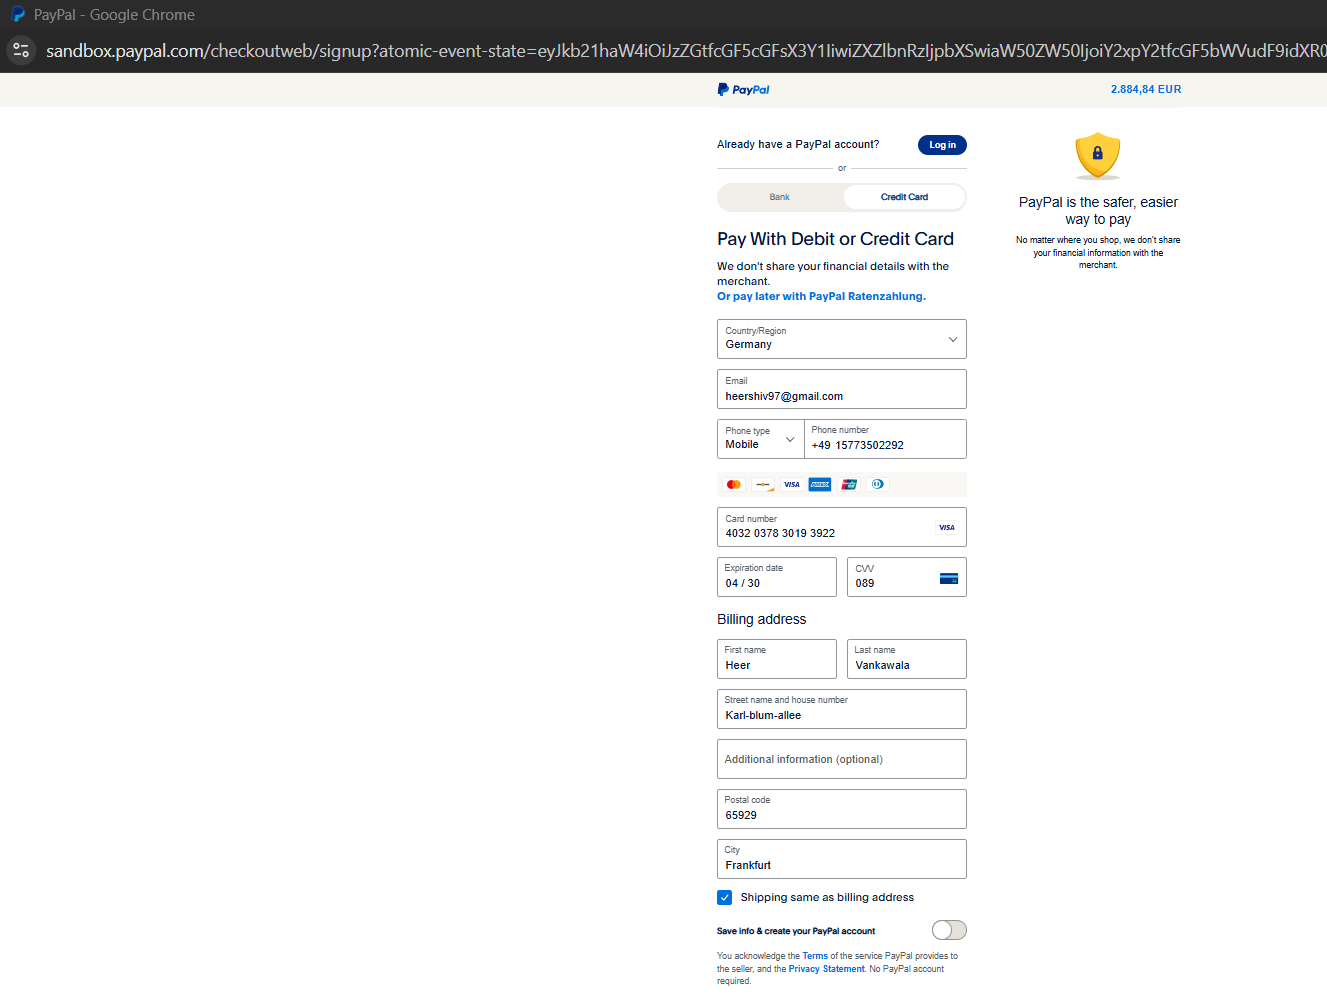
\includegraphics[width=0.5\textwidth]{../images/Proceed_payment_Paypal.png} }}
    \vspace{0.01\textwidth}
    \caption{Paypal Payment Processing}
    \label{fig:Webshop_6}
\end{figure}


\vphantom{ }\\
\begin{figure}[H]
    \centering
    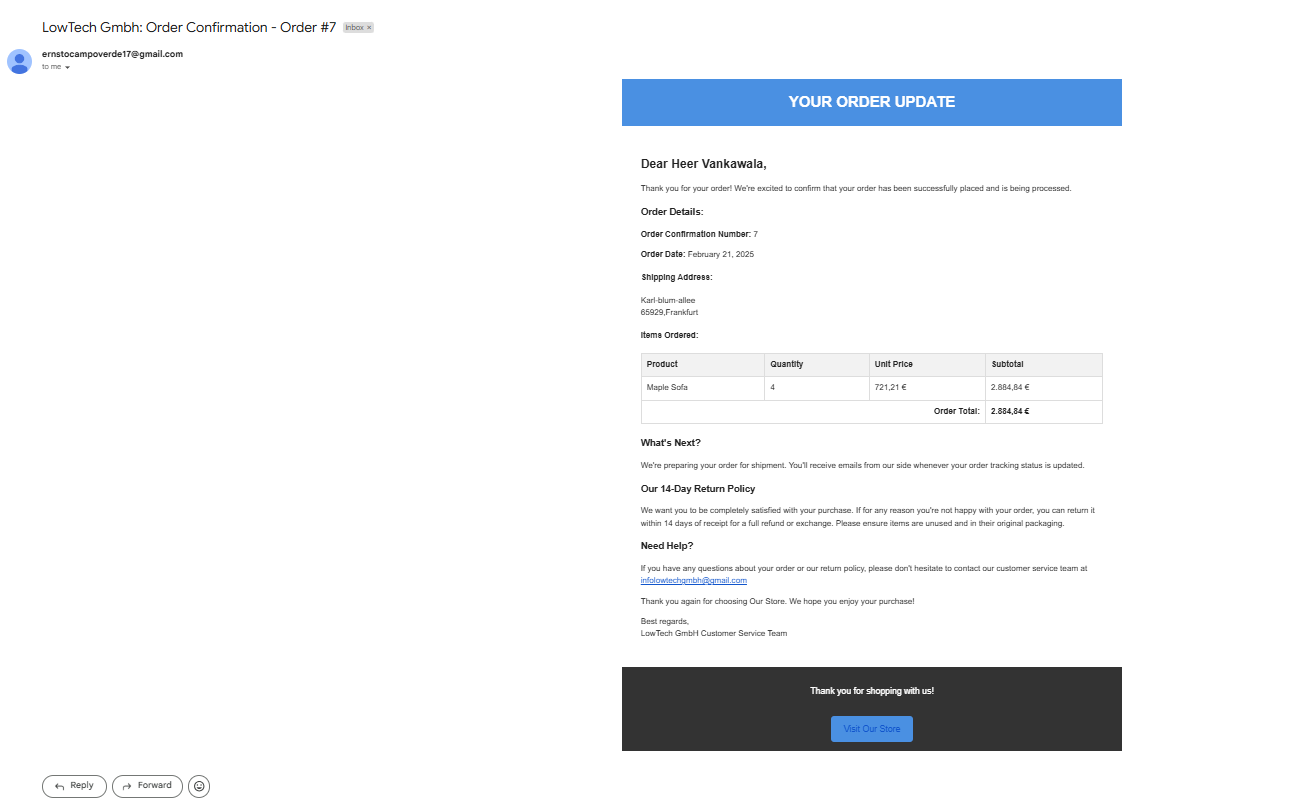
\includegraphics[width=0.8\textwidth]{../images/Shipment_email.png}
    \vspace{0.01\textwidth}
    \caption{Shipment Notification Email Received for Order}
    \label{fig:Webshop_7}
\end{figure}

\vphantom{ }\\
\begin{figure}[H]
    \centering
    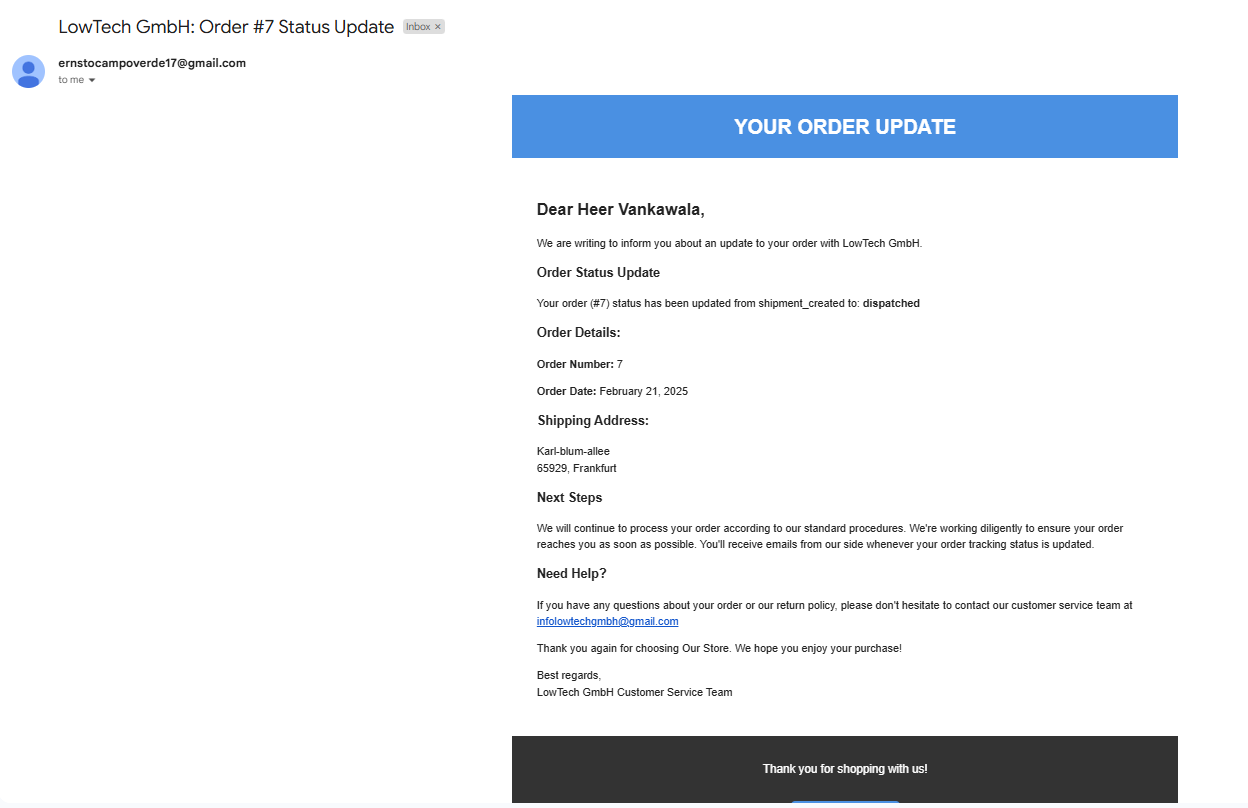
\includegraphics[width=0.8\textwidth]{../images/dispatched_email.png}
    \vspace{0.01\textwidth}
    \caption{Order Dispatched Email Received After Status Change}
    \label{fig:Webshop_8}
\end{figure}

\vphantom{ }\\
\begin{figure}[H]
    \centering
    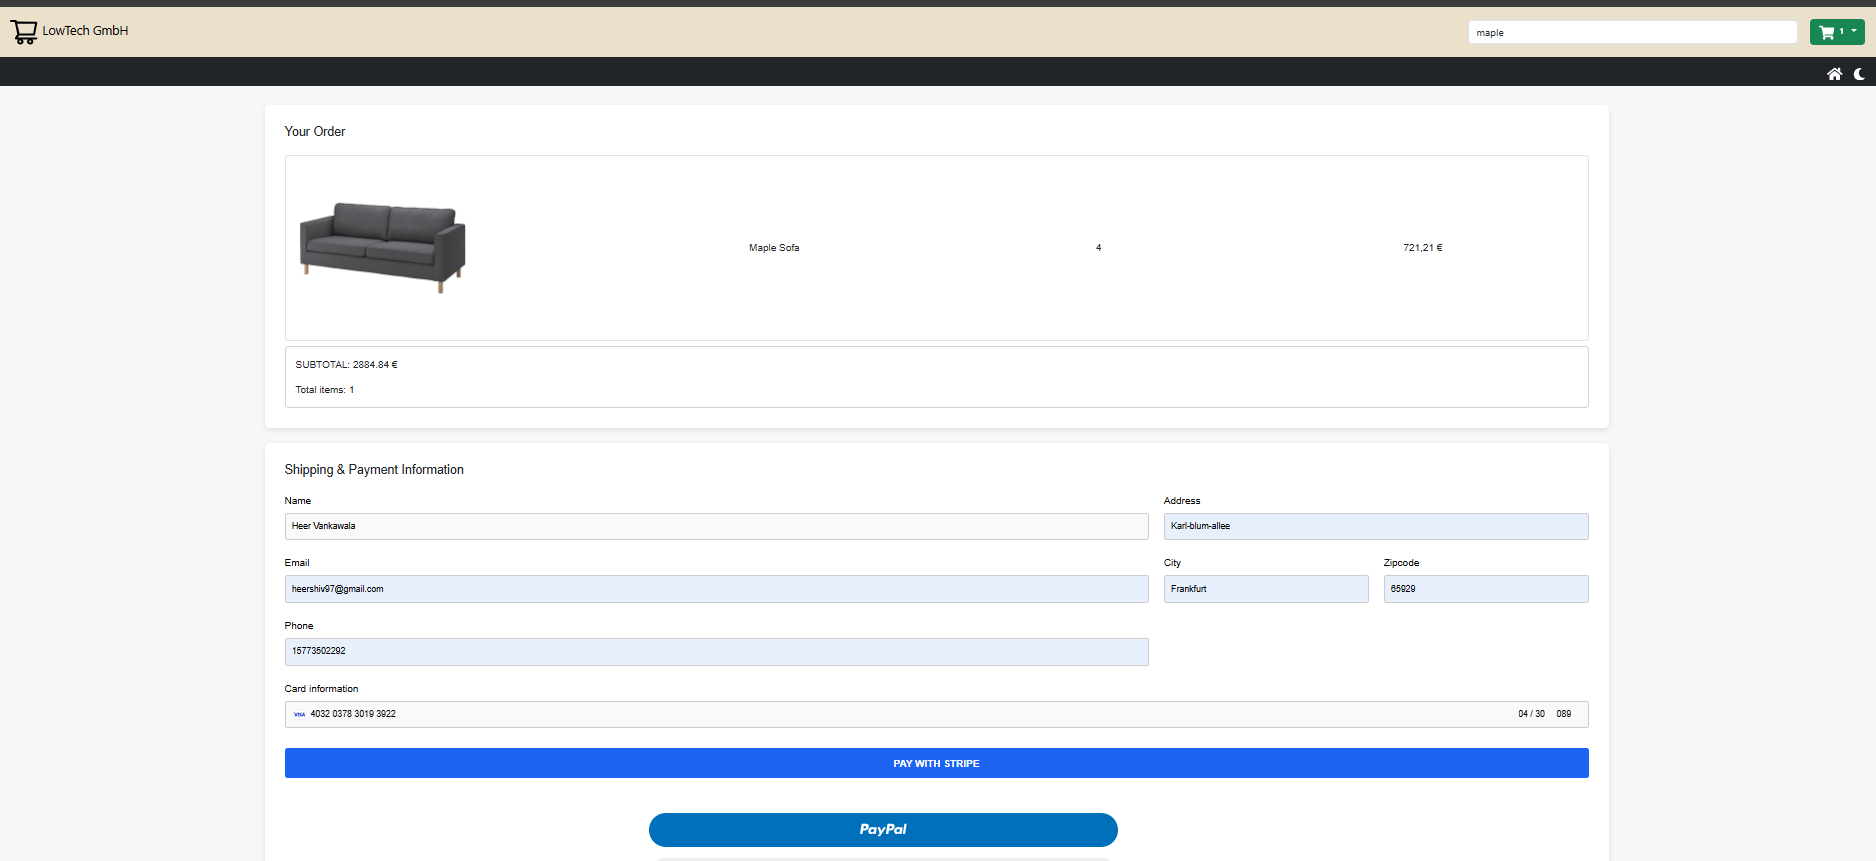
\includegraphics[width=0.8\textwidth]{../images/Payment_Stripe.png}
    \vspace{0.01\textwidth}
    \caption{Order Placed with Stripe Payment Method}
    \label{fig:Webshop_9}
\end{figure}
\vphantom{ }\\
\begin{figure}[H]
    \centering
    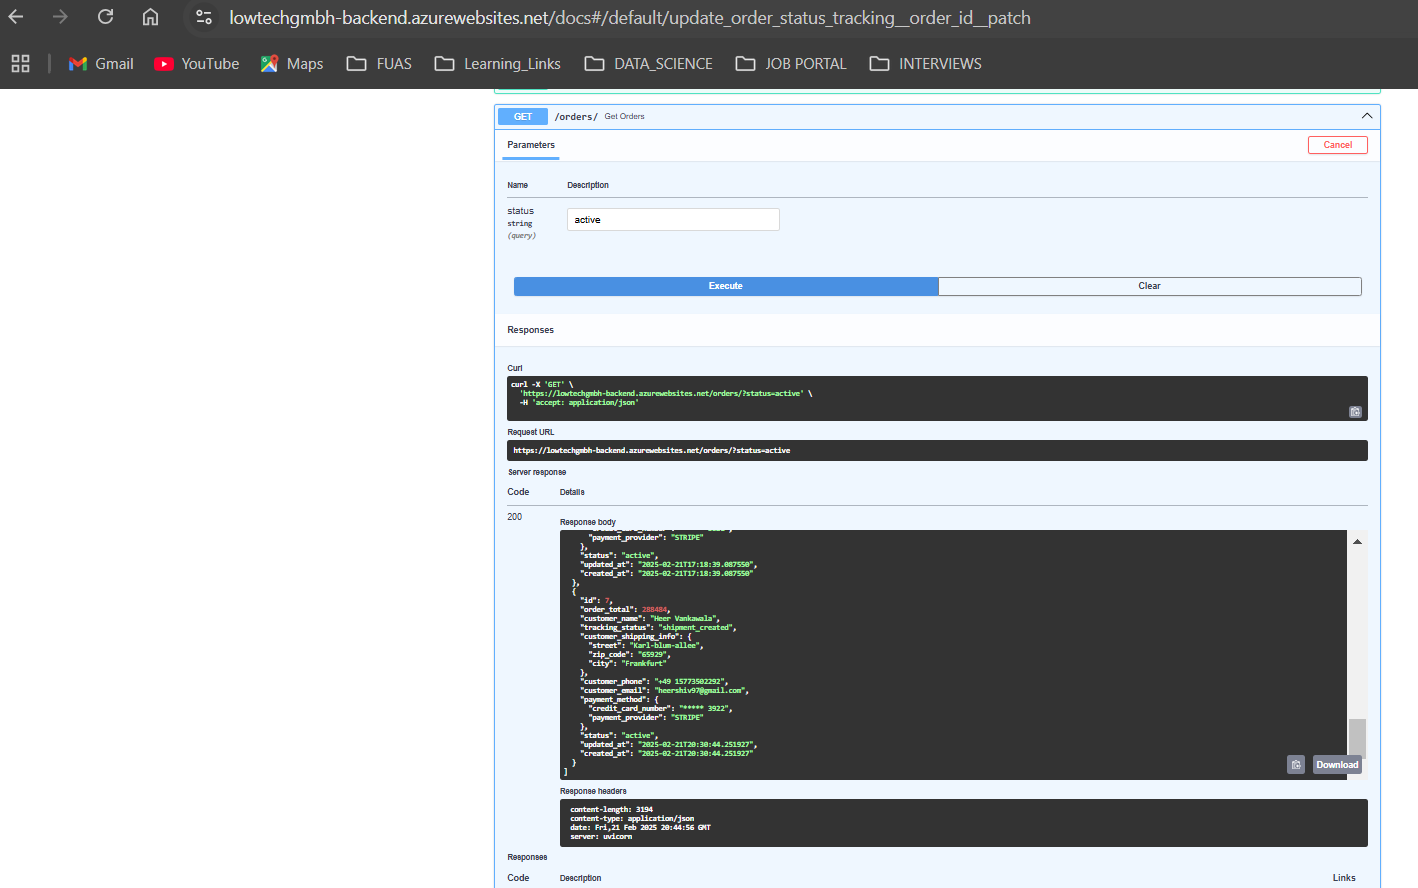
\includegraphics[width=0.8\textwidth]{../images/Get_Order_API.png}
    \vspace{0.01\textwidth}
    \caption{Order Data Retrieved Through Fast API for All Placed Orders}
    \label{fig:Webshop_10}
\end{figure}


\section{Critical Analysis}

In general the application conforms to the specification of the client. Neverhteless, in hindsight, some areas of the code, infrastructure, and development process could have been improved.
\begin{itemize}
    \item The base project for the front end used vanila JavaScript and no state management library. Initially to get the store up and running fast is perfect.
          But, once we need to add more functionality and the state management becomes more complex, we could have beneffited from the inclusion of a stronger type system. And a dedicated state management solution.
          Even on the first stages of integration, the lack of types makes it more difficult to integrate with the backend.
    \item The choice of 3 different services to run the application might have been more complex than what was needed.
          In theory either Azure App Service and Static Web apps could have easily handled the entirety of the application.
    \item Once we start scaling up, having three different services scaling independently even thouhg is more flexible, could result in bigger expenses,
          since all network traffic and DNS queries, even internally are billed. This is a situation that becomes less of a problem if all components are in a single service.

    \item The management of the database becomes more difficult once you host the server on a private virtual cloud. We had to create a virtual machine to act as a proxy for migrations and seeding the database.
\end{itemize}
\subsection{Cloud Service Evaluation}

In general the configuration of the services was simple enough. Nevbertheless there were some setbvacks associated to the type of subscription we were using.
All services have auto-scaling capabilities, which can be enabled on demand, and configured acording to the aplications needs.


\subsubsection{Azure Static Web Apps}
In this case we are using the Free SKU. The main disadvantage of the Free SKU is that is very limited in terms of throughput and connections to the client.
Nevertheless this service can be upgraded to use "enterprise-grade ege" meaning that Azure will automatically cache the website on edge servers making it fast and easy to deliver to clients.

This service does not support traditional autoscaling since we are not rendering on the server. The client connects to the backend using http.

One of the disadvantages is thet even though it allows for integration options with APIs and even databases, it is clear that we will have to architect the application to only be tailored to use this services under Azyres paradigms.

Another disadvantage is that it requires its own resource group and own subnet.\\
\begin{figure}[H]
    \centering
    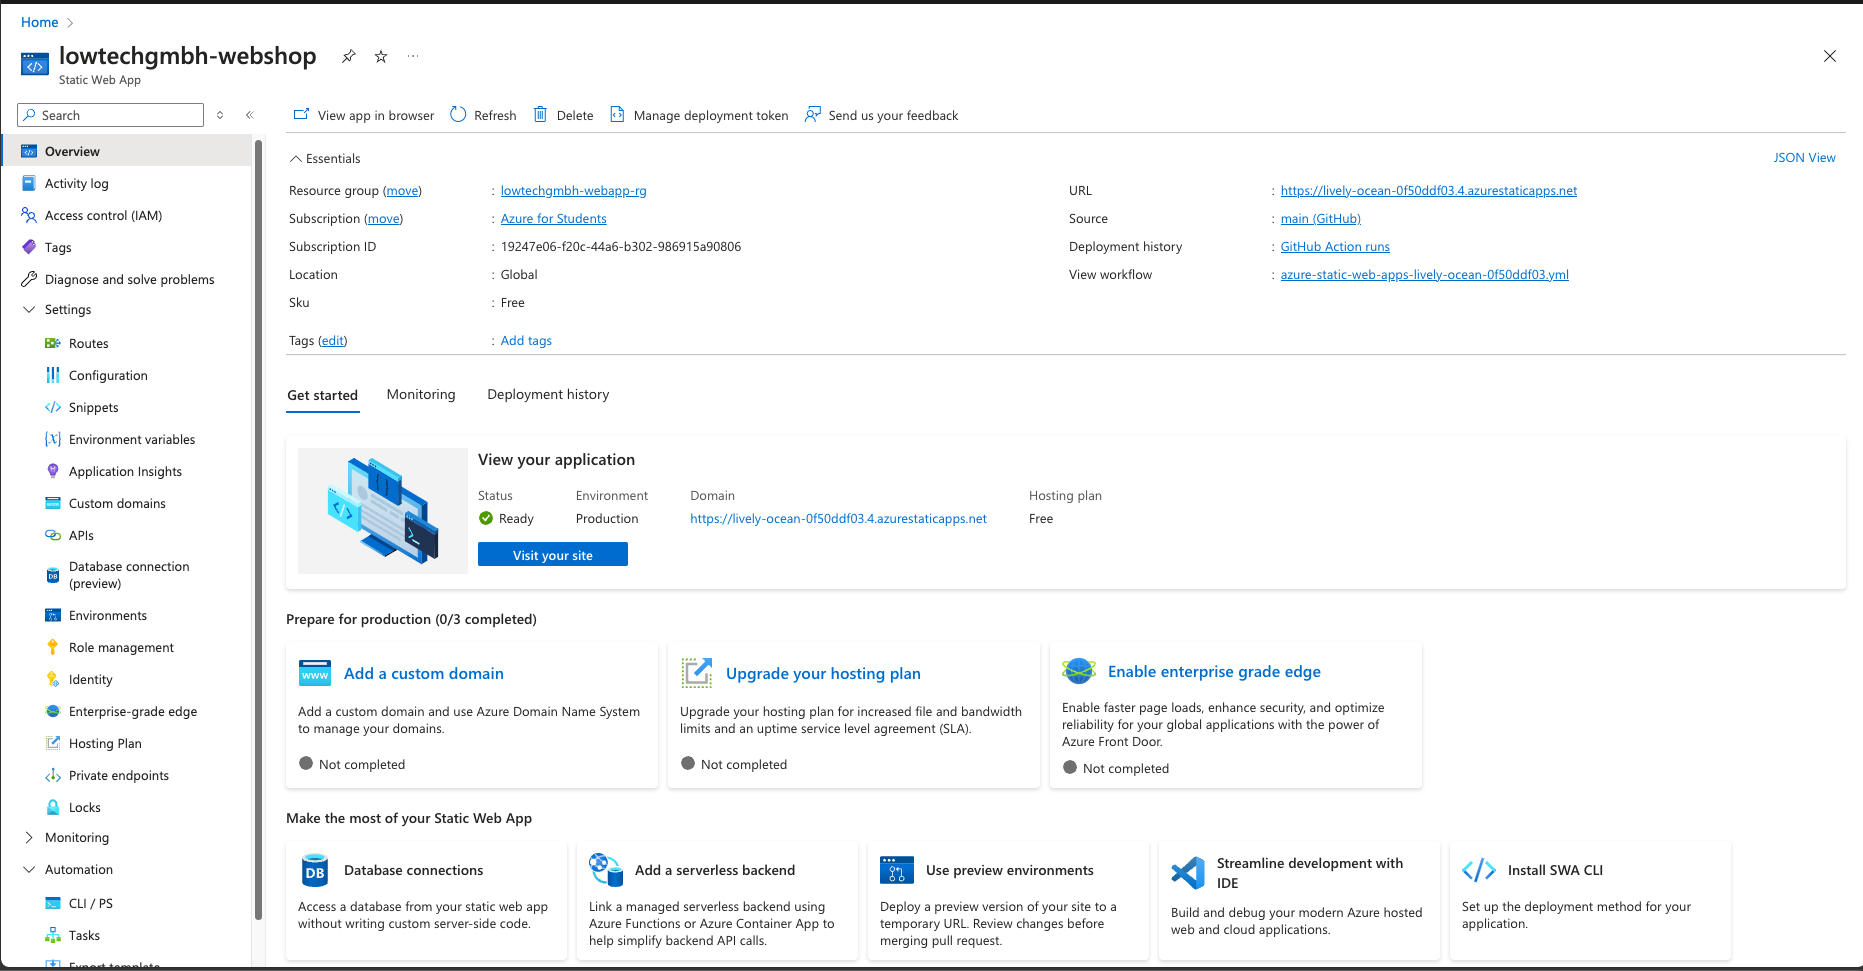
\includegraphics[width=0.8\textwidth]{../images/frontend_azure.png}
    \vspace{0.01\textwidth}
    \caption{Azure Static Web Apps Dashboard}
    \label{fig:frontend_azure}
\end{figure}


\subsubsection{Azure App Service}

This service was used due to its versatility in deploying any type of web applications. To avoid extra costs associated to a private image registry,
to handle deploys we are packaging all the code and artifacts in the github runner and publishing to our application.

One of the disadvantages is the price, once we start using the more advanced features and more compute, the service scales rapidly in cost.\\

\begin{figure}[H]
    \centering
    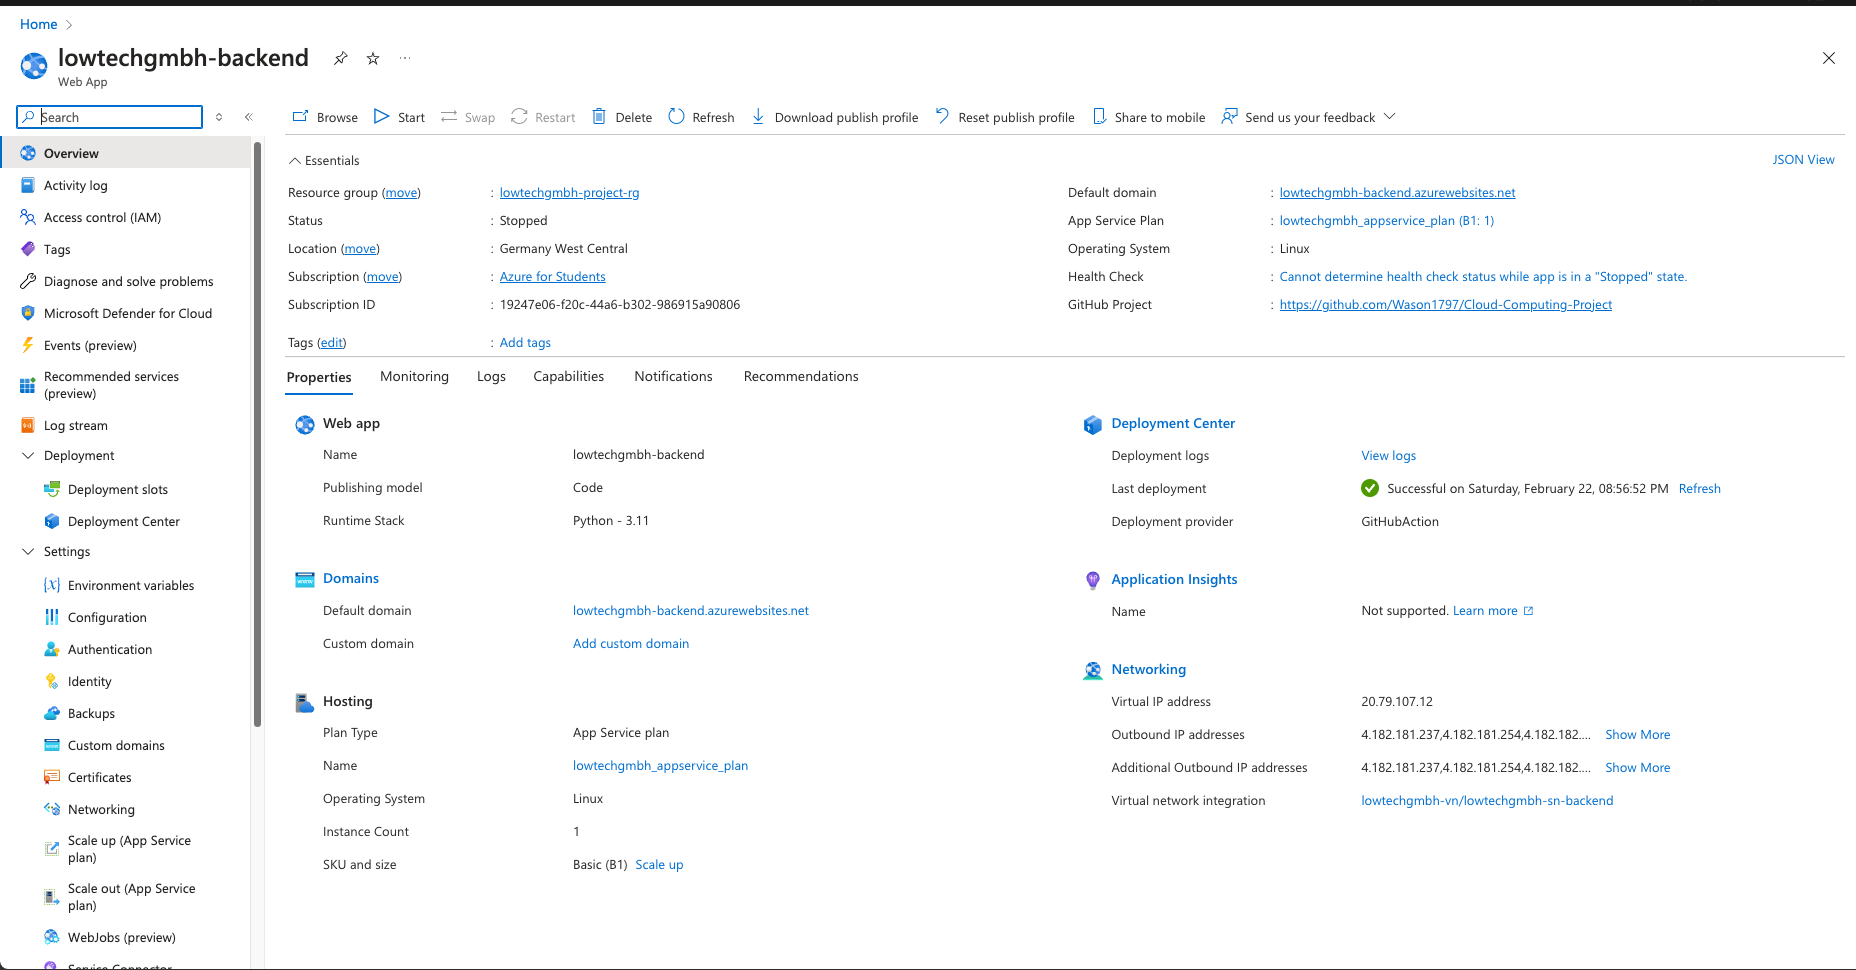
\includegraphics[width=0.8\textwidth]{../images/backend_azure.png}
    \vspace{0.01\textwidth}
    \caption{Azure App Service Dashboard}
    \label{fig:backend_azure}
\end{figure}


\subsubsection{Azure PostgreSQL Flexible Server}

This is one of the more reasonable options to deploy a database server in Azure, given that the Free tier is quite capable. It also offers automatic maintenance and backups.

In this case, one of the disadvantages is the access complexity if we decide to host it on a VPC and not have a public IP.\\

\begin{figure}[H]
    \centering
    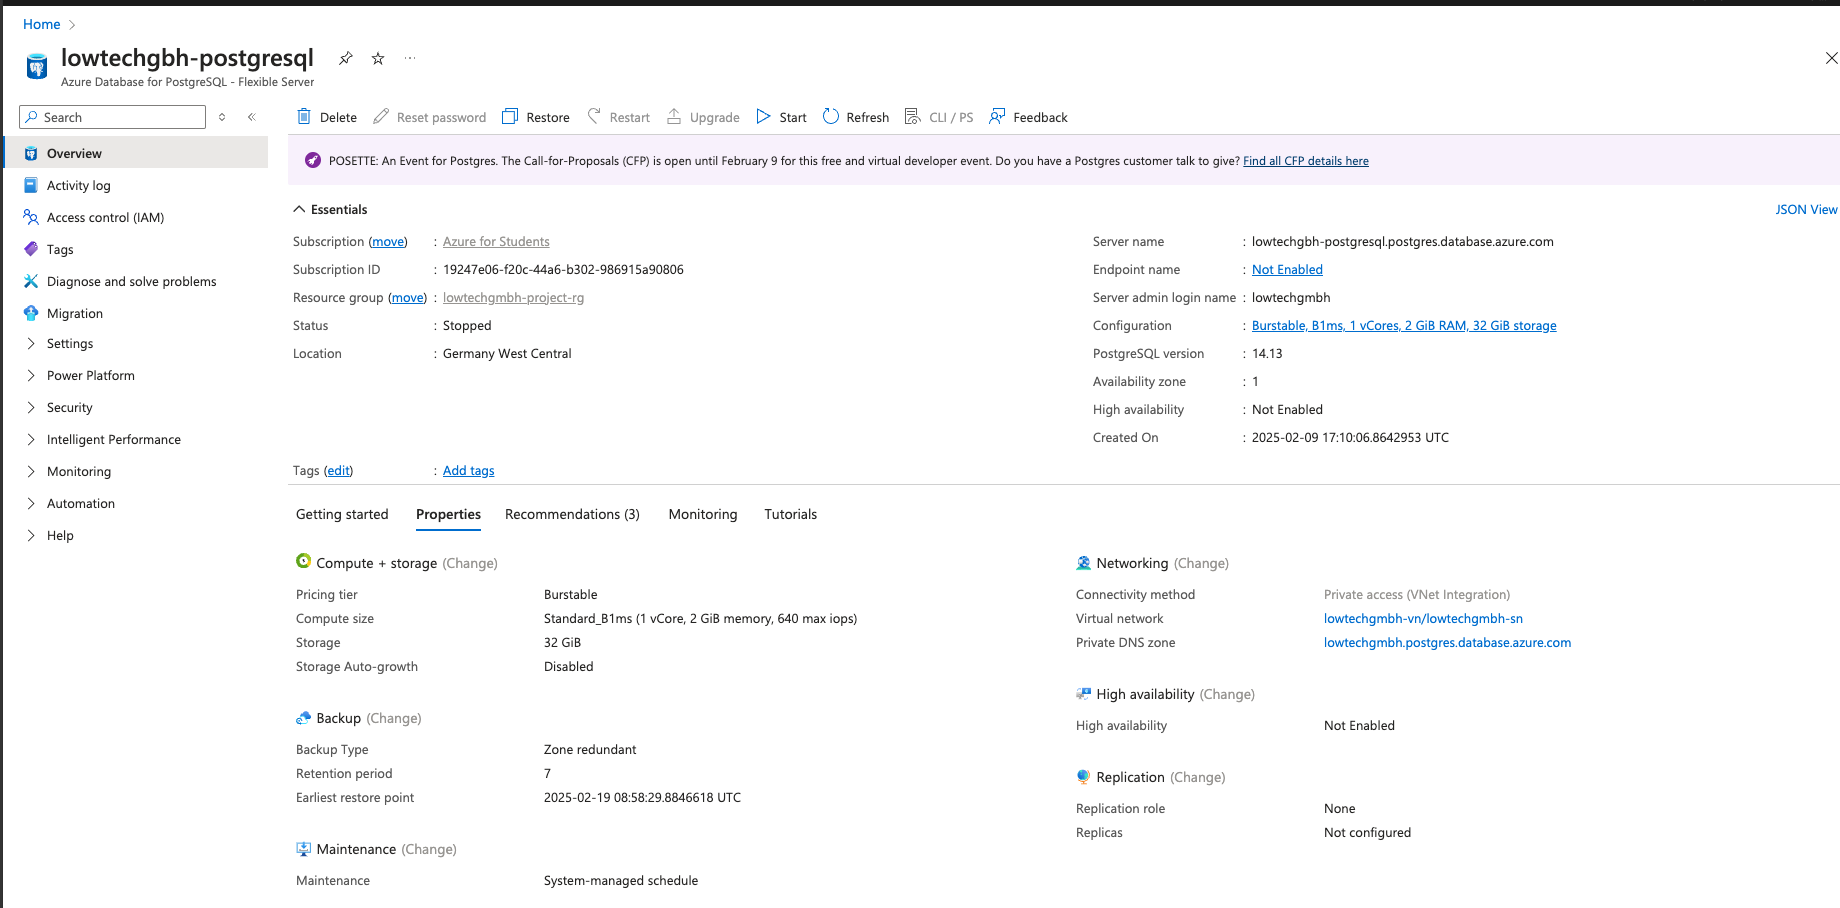
\includegraphics[width=0.8\textwidth]{../images/database_azure.png}
    \vspace{0.01\textwidth}
    \caption{Azure PostgreSQL Flexible Server Dashboard}
    \label{fig:database_azure}
\end{figure}


\subsection{Architectural Decisions}

\begin{itemize}
    \item The frontend application uses a really basic component driven approach and segregates all API comunication logic to its own folder.
    \item In the backend we decided to have 2 simple layers, the database access layer, and the presentation layer i.e. The endpoints.
          Given the time constraints, and the scope of the project we did not divide the code further.
    \item We used FastAPI in the backend given its asynchronous nature, meaning a more efficient use of CPU resources, and the ability to schedule background tasks to send emails out of the box.
    \item In general this application is stil limited by the scale of the database, given that we are not using a microservice approach or have a database that supports sharding.
          Nevertheless, we feel that for a webshop which needs to handle orders, transaction integrity is more important than data replication. Furthermore, given the flexible nature of the cloud, we could scale the server vertically if there is the need.

\end{itemize}


\section{Repository Documentation}
\subsection{GitHub Structure}

The team configured the following repository: https://github.com/Helly2010/Cloud-Computing-Project.

\begin{enumerate}
    \item \textbf{Branching Strategy:} \newline
          The project follows a simple main branch strategy where all contributors work directly on the main branch.
          This ensures seamless integration without managing multiple branches. All changes should be committed with meaningful messages.
          Code should be reviewed and tested before pushing to the main branch.

    \item \textbf{Continuous Integration/Continuous Deployment:}
          \begin{itemize}
              \item \textbf{Continuous Deployment (CD):}

                    Once the CI stage passes successfully, the application is automatically deployed to the appropriate environment. This process includes:
                    \begin{itemize}
                        \item Deploying to a staging environment for final testing.
                        \item Running automated acceptance tests before production deployment.
                        \item Deploying to production with rollback mechanisms in case of failure.
                    \end{itemize}

          \end{itemize}
\end{enumerate}


\subsection{Contributions}
\begin{figure}[htbp]
    \centering
    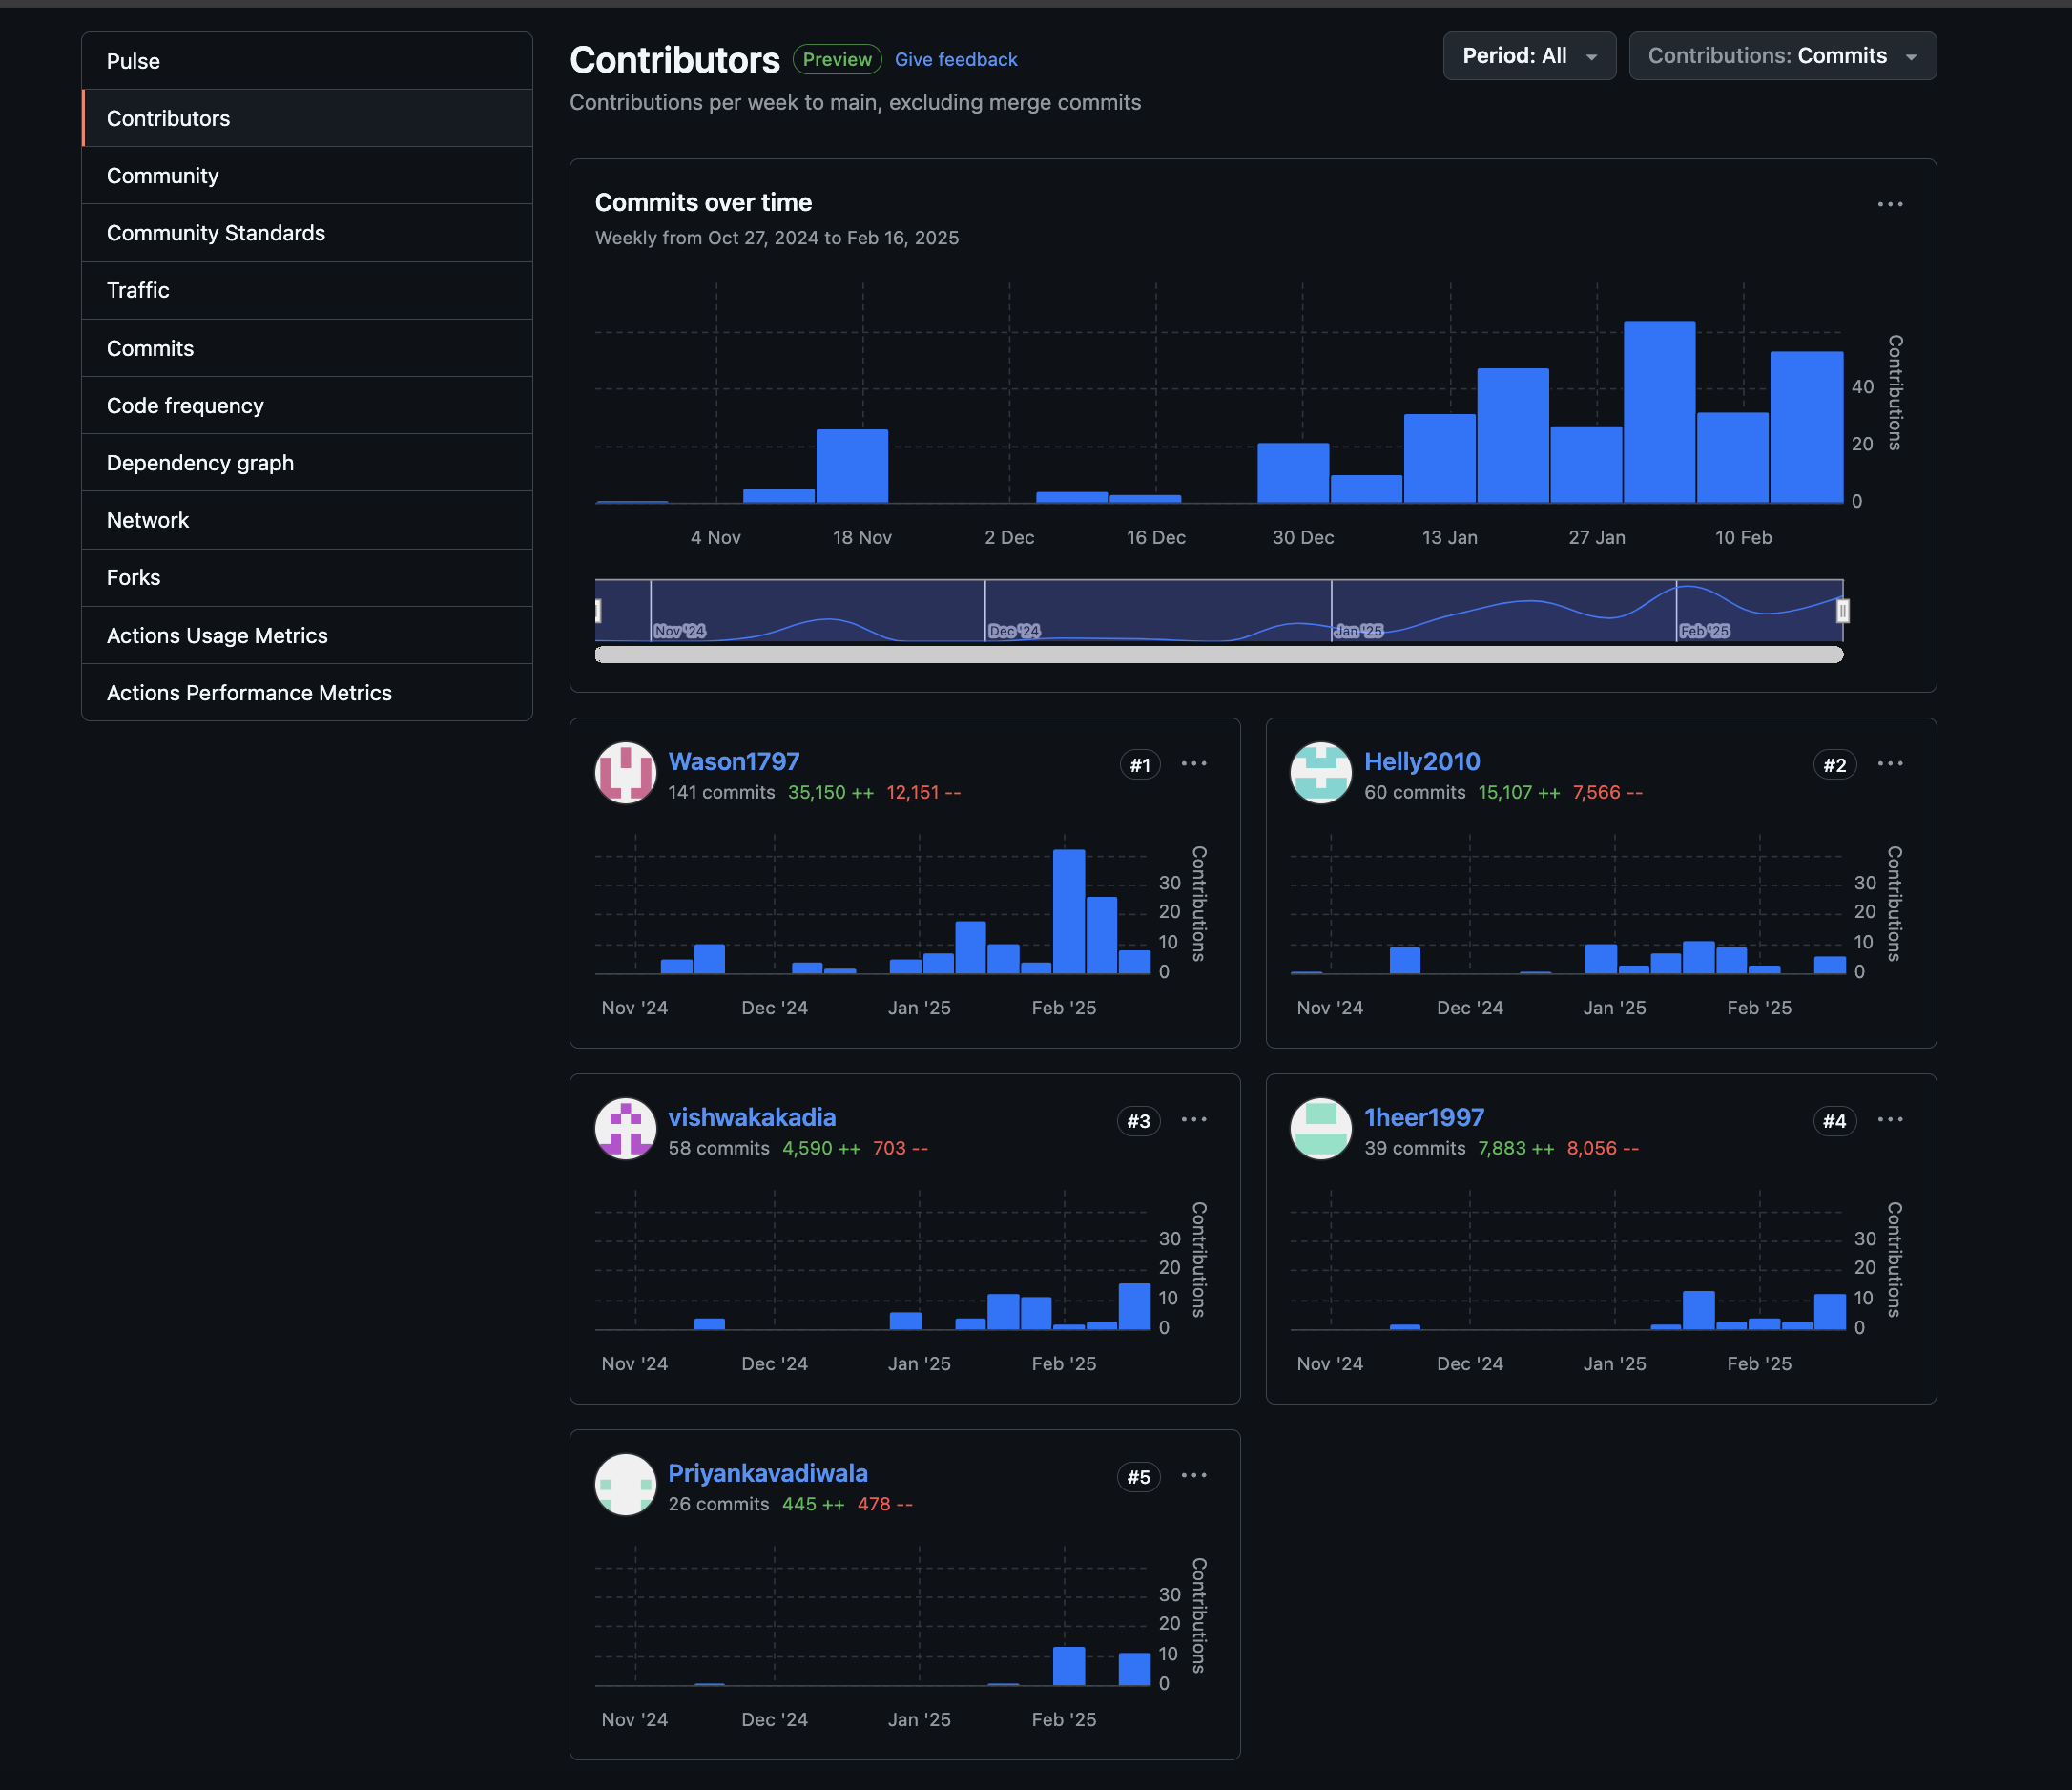
\includegraphics[width=0.7\textwidth]{../images/contributions.png}
    \vspace{0.01\textwidth}
    \caption{Contribution Stats in GitHub}
    \label{fig:contributions}
\end{figure}

\vphantom{}\\

\begin{table}[htbp]

    \begin{tabular}{|p{0.7\textwidth}|p{0.3\textwidth}|}
        \hline
        \textbf{Topic}    & \textbf{Contributor}      \\
        \hline
        Introduction and Objectives of Cloud Implementation  \newline
        Repository Documentation & Priyanka Vadiwala         \\
        \hline
        Implementation Process  And Critical Analysis
                       & Wladymir Brborich-Herrera \\
        \hline
        add \newline
        add               & Heer Vankawala            \\
        \hline
        add \newline
        add               & Hellyben Shah             \\
        \hline
        Application Design, System Diagrams              & Vishwaben Kakadiya        \\
        \hline
    \end{tabular}
    \caption{Contribution Table}
    \label{tab:contribution}
\end{table}

\section{Conclusion}
\subsection{Project Outcomes}

At the end of the project we had a 3 tier cloud native application running.
Furthermore, we have infrastructure templates to recreate this particular setup with minimal manual configuration.
The team also implemented a database migration system to track changes to the tables and to actually seed the initial data without much effort.
All services have the possibility to scale horizontally, and are easily configurable. Nevertheless the architecture of the project could have been much simpler.
As it was pointed out in the critical analysis of our project, services like Azure static web apps offer the possibility to deploy all 3 layers in one single service.
Some of them even include their own MySQL database. We believe that it could be a more cost effective way, but at the cost of flexibility.
Since all the application will be tailored to a single service.


\subsection{Future Enhancements}
For production readiness a lot of polish work is needed, specially in the order handling and tracking, not to mention security and user management.
Nevertheless, in the infrastructure side, it is a matter of changing the SKUs and autoscaling configurations to something more appropriate depending on the expected load.
Inherently the system runs in a private network inside the cloud provider, and it provides https certificates out of the box.
If in the future the cost assesment reveals that the choice of servies was on the expensive side, we could at least consolidate the presentation and business logic layers in one service.


\begin{thebibliography}{9}

    \bibitem{AppServiceplan}
    Microsoft,
    \emph{Azure App Service plan overview},
    2024, Available:
    \url{https://learn.microsoft.com/en-us/azure/app-service/overview-hosting-plans}.

    \bibitem{MicrosoftAzureSubscriptionLimits}
    Microsoft,
    \emph{Azure subscription and service limits, quotas, and constraints},
    2024, Available:
    \url{https://learn.microsoft.com/en-us/azure/azure-resource-manager/management/azure-subscription-service-limits}.

    \bibitem{azurepricingcalculator}
    Microsoft, Available:
    \emph{Azure Pricing Calculator}, 2024,
    \url{https://azure.microsoft.com/de-de/pricing/calculator/}.

    \bibitem{MicrosoftAzurePythonConfig}
    Microsoft,
    \emph{Configure Linux Python apps - Azure App Service},
    2024, Available:
    \url{https://learn.microsoft.com/en-us/azure/app-service/configure-language-python}

    \bibitem{azurestaticwebapps}
    Microsoft,
    \emph{What is Azure Static Web Apps?}, 2024,
    Available: \url{https://learn.microsoft.com/en-us/azure/static-web-apps/overview}.

    \bibitem{azuredatabase}
    Microsoft,
    \emph{Azure Database for PostgreSQL – Flexible Servers}, 2024,
    Available: \url{https://learn.microsoft.com/de-de/azure/postgresql/flexible-server/overview}.

    \bibitem{azurevirtualscale}
    Microsoft,
    \emph{What are Virtual Machine Scale Sets?}, 2024,
    Available: \url{https://learn.microsoft.com/en-us/azure/virtual-machine-scale-sets/overview}.

\end{thebibliography}
\end{document}

